
\documentclass{llncs}

%%%(20 pages max, must be anonymized)
%% Conference information

\usepackage{mathrsfs}
\usepackage{blindtext}
\usepackage{minted}
\usepackage{eqnarray}
\usepackage{amssymb}
\usepackage{mathtools}

\newif\ifdraft\drafttrue
%\newif\ifdraft\draftfalse
\ifdraft
\newcommand{\anthony}[1]{\color{red} {AL: #1 :LA} \color{black}}
\newcommand{\zhilin}[1]{\color{brown} {ZL: #1 :LZ} \color{black}}
\newcommand{\tl}[1]{\color{blue} {TL: #1 :LT} \color{black}}
\newcommand{\mat}[1]{\color{cyan} {MH: #1 :HM} \color{black}}
\newcommand{\philipp}[1]{\color{magenta} {PR: #1 :PR} \color{black}}
\newcommand{\zhilei}[1]{\color{violet} {ZLH: #1 :HZL} \color{black}}
\else
\newcommand{\anthony}[1]{}
\newcommand{\zhilin}[1]{}
\newcommand{\tl}[1]{}
\newcommand{\mat}[1]{}
\newcommand{\zhilei}[1]{}
\fi


%\newcommand{\ASSERT}[1]{\textsf{assert}\left(#1\right)}
%%%%%%%%%% End TeXmacs macros



%!TEX root = main.tex

\newcommand{\brac}[1]{\left( #1 \right)}
\newcommand{\tup}[1]{\left( #1 \right)}
\newcommand{\set}[1]{\{ #1 \}}
\newcommand{\sequence}[2]{(#1, \ldots, #2)}
\newcommand{\couple}[2]{(#1,#2)}
\newcommand{\pair}[2]{(#1,#2)}
\newcommand{\triple}[3]{(#1,#2,#3)}
\newcommand{\quadruple}[4]{(#1,#2,#3,#4)}
\newcommand{\tuple}[2]{(#1,\ldots,#2)}
\newcommand{\Nat}{\ensuremath{\mathbb{N}}}
\newcommand{\Rat}{\ensuremath{\mathbb{Q}}}
\newcommand{\Rea}{\ensuremath{\mathbb{R}}}
\newcommand{\Zed}{\ensuremath{\mathbb{Z}}}
%\newcommand{\true}{\top}
%\newcommand{\false}{\perp}
\newcommand{\bottom}{\perp}
%% \newcommand{\powerset}[1]{{\cal P}(#1)}
\newcommand{\npowerset}[2]{{\cal P}^{#1}(#2)}
\newcommand{\finitepowerset}[1]{{\cal P}_f(#1)}
\newcommand{\level}[2]{L_{#1}(#2)}
\newcommand{\card}[1]{\mbox{card}(#1)}
\newcommand{\range}[1]{\mathtt{ran}(#1)}
\newcommand{\astring}{s}

\newcommand{\Cc}{\mathcal{C}}


\newcommand {\notof}{\ensuremath{\neg}}
\newcommand {\myand}{\ensuremath{\wedge}}
\newcommand {\myor}{\ensuremath{\vee}}
\newcommand {\mynext}{\mbox{{\sf X}}}
\newcommand {\until}{\mbox{{\sf U}}}
\newcommand {\sometimes}{\mbox{{\sf F}}}
\newcommand {\previous}{\mynext^{-1}}
\newcommand {\since}{\mbox{{\sf S}}}
\newcommand {\fminusone}{\mbox{{\sf F}}^{-1}}
\newcommand {\everywhere}[1]{\mbox{{\sf Everywhere}}(#1)}



\newcommand{\aatomic}{{\rm A}}
\newcommand{\aset}{X}
\newcommand{\asetbis}{Y}
\newcommand{\asetter}{Z}

\newcommand{\avarprop}{p}
\newcommand{\avarpropbis}{q}
\newcommand{\avarpropter}{r}
\newcommand{\varprop}{{\rm PROP}} % Set of atomic propositions (for a given logic)

% formulae

\newcommand{\aformula}{\astateformula} % a formula
\newcommand{\aformulabis}{\astateformulabis} % another formula (when at least 2 are present)
\newcommand{\aformulater}{\astateformulater} % another formula (when at least 3 are present)
\newcommand{\asetformulae}{X}
\newcommand{\subf}[1]{sub(#1)}

\newcommand{\aautomaton}{{\mathbb A}}
\newcommand{\aautomatonbis}{{\mathbb B}}

\newcommand {\length}[1] {\ensuremath{|#1|}}



% Equivalences
\newcommand{\egdef}{\stackrel{\mbox{\begin{tiny}def\end{tiny}}}{=}} % =def=
\newcommand{\eqdef}{\stackrel{\mbox{\begin{tiny}def\end{tiny}}}{=}} % =def=
\newcommand{\equivdef}{\stackrel{\mbox{\begin{tiny}def\end{tiny}}}{\equivaut}} % <=def=>
\newcommand{\equivaut}{\;\Leftrightarrow\;}

\newcommand{\ainfword}{\sigma}

\newcommand{\amap}{\mathfrak{f}}
\newcommand{\amapbis}{\mathfrak{g}}

\newcommand{\step}[1]{\xrightarrow{\!\!#1\!\!}}
\newcommand{\backstep}[1]{\xleftarrow{\!\!#1\!\!}}

\newcommand {\aedge}[1] {\ensuremath{\stackrel{#1}{\longrightarrow}}}
\newcommand {\aedgeprime}[1] {\ensuremath{\stackrel{#1}{\longrightarrow'}}}
\newcommand {\afrac}[1] {\ensuremath{\mathit{frac}(#1)}}
\newcommand {\cl}[1] {\ensuremath{\mathit{cl}(#1)}}
\newcommand {\sfc}[1] {\ensuremath{\mathit{sfc}(#1)}}
\newcommand {\dunion} {\ensuremath{\uplus}}
\newcommand {\edge} {\ensuremath{\longrightarrow}}
\newcommand {\emptyword}{\ensuremath{\epsilon}}
\newcommand {\floor}[1] {\ensuremath{\lfloor #1 \rfloor}}
\newcommand {\intersection} {\ensuremath{\cap}}
\newcommand {\union} {\ensuremath{\cup}}
\newcommand {\vals}[2] {\ensuremath{\mathit{val}_{#2}(#1)}}



\newcommand {\pspace} {\textsc{pspace}}
\newcommand {\nlogspace} {\textsc{nlogspace}}
\newcommand {\logspace} {\textsc{logspace}}
\newcommand {\expspace} {\textsc{expspace}}
\newcommand {\np} {\textsc{np}}
\newcommand {\threeexptime} {\textsc{3exptime}}
\newcommand {\polytime} {\textsc{p}}
\newcommand{\twoexpspace}{\textsc{2expspace}}
\newcommand{\threeexpspace}{\textsc{3expspace}}
\newcommand {\nexptime} {\textsc{nexptime}}



\newcommand{\aalphabet}{\Sigma}     % an alphabet, A is already used for atoms
\newcommand{\aword}{\mathfrak{u}}
\newcommand{\awordbis}{\mathfrak{v}}



\newcommand{\aassertion}{P}
\newcommand{\aassertionbis}{Q}
\newcommand{\aexpression}{e}
\newcommand{\aexpressionbis}{f}
\newcommand{\avariable}{\mathtt{x}}
\newcommand{\uniquevar}{\mathtt{u}}
\newcommand{\uniquevarbis}{\mathtt{v}}
\newcommand{\avariablebis}{\mathtt{y}}
\newcommand{\avariableter}{\mathtt{z}}
\newcommand{\nullconstant}{\mathtt{null}}
\newcommand{\nilvalue}{nil}
\newcommand{\emptyconstant}{\mathtt{emp}}
\newcommand{\infheap}{\mathtt{inf}}
\newcommand{\saturated}{\mathtt{Saturated}}

\newcommand{\astateformula}{\phi}
\newcommand{\astateformulabis}{\psi}
\newcommand{\astateformulater}{\varphi}
%%
\newcommand{\separate}{\ast}
\newcommand{\sep}{\separate}
\newcommand{\size}{\mathtt{size}}
\newcommand{\sizeeq}[1]{\mathtt{size} \ = \ #1}
\newcommand{\alloc}[1]{\mathtt{alloc}(#1)}
\newcommand{\allocb}[2]{\mathtt{alloc}^{-1}[#2](#1)}
\newcommand{\isol}[1]{\mathtt{isoloc}(#1)}
\newcommand{\icell}{\mathtt{isocell}}
\newcommand{\malloc}{\mathtt{malloc}}
\newcommand{\cons}{\mathtt{cons}}
\newcommand{\new}{\mathtt{new}}
\newcommand{\free}[1]{\mathtt{free} #1}
\newcommand{\maxform}[1]{\mathtt{maxForms}(#1)}
\newcommand{\locations}[1]{\mathtt{loc}(#1)}
\newcommand{\values}{\mathtt{Val}}
\newcommand{\aheap}{\mathfrak{h}}
\newcommand{\avaluation}{\mathfrak{V}}
\newcommand{\heaps}{\mathcal{H}}
\newcommand{\astore}{\mathfrak{s}}
\newcommand{\stores}{\mathcal{S}}
\newcommand{\amodel}{\mathfrak{M}}
\newcommand{\alabel}{\ell}

\newcommand{\aprogram}{\mathtt{PROG}}
\newcommand{\programs}{\mathtt{P}}
\newcommand{\ctprograms}{\programs^{ct}}
\newcommand{\aninstruction}{\mathtt{instr}}
\newcommand{\ainstruction}{\mathtt{instr}}
\newcommand{\instructions}{\mathtt{I}}
\newcommand{\aguard}{\ensuremath{g}}
\newcommand{\guards}{\ensuremath{G}}
\newcommand{\domain}[1]{\mathtt{dom}(#1)}
\newcommand{\memory}{\stores\times\heaps}
\newcommand{\skipinstruction}{\mathtt{skip}}

\newcommand{\execution}{\mathtt{comp}}
\newcommand{\aux}{\mathtt{embd}}
\newcommand{\runof}{run}
\newcommand{\anexecution}{e}


\newcommand{\aletter}{\ensuremath{a}}
\newcommand{\aletterbis}{\ensuremath{b}}
\newcommand{\alocation}{\mathfrak{l}}

\newcommand{\pointsl}[1]{\stackrel{#1}{\hookrightarrow}}
\newcommand{\ppointsl}[1]{\stackrel{#1}{\mapsto}}
\newcommand{\ourhook}[1]{\stackrel{#1}{\hookrightarrow}}
\newcommand{\ltrue}{{\sf true}}
\newcommand{\lfalse}{{\sf false}}


\newcommand{\variables}{\mathtt{FVAR}}
\newcommand{\pvariables}{\mathtt{PVAR}}
\newcommand{\secvariables}{\mathtt{SVAR}}
\newcommand{\logique}[1]{\mathtt{FO}(#1)}



\newcommand{\atranslation}{\mathfrak{t}}
\newcommand{\nbpred}[1]{\widetilde{\sharp #1}}
\newcommand{\nbpredstar}[1]{\widetilde{\sharp #1}^{\star}}
\newcommand{\isolated}{\mathtt{isol}}
\newcommand{\stdmarks}{\mathtt{envir}}
\newcommand{\relation}[1]{\mathtt{relation}_{#1}}
\newcommand{\freevar}{\mathtt{FV}}
\newcommand{\notonmark}{\mathtt{notonenv}}
\newcommand{\InVal}[1]{\mathtt{InVal}\!\left(#1\right)}
\newcommand{\NotOnEnv}[1]{\mathtt{NotOnEnv}\!\left(#1\right)}
\newcommand{\PartOfVal}[1]{\mathtt{PartOfVal}\!\left(#1\right)}
%\newcommand{\nbpreds}[3]{\sharp #1 \geq #2}
\newcommand{\defstyle}[1]{{\emph{#1}}}

\newcommand{\cut}[1]{}
\newcommand{\interval}[2]{[#1,#2]}
\newcommand{\buniquevar}{\overline{\uniquevar}}
\newcommand{\bbuniquevar}{\overline{\overline{\uniquevar}}}
\newcommand{\magicwand}{\mathop{\mbox{$\mbox{$-~$}\!\!\!\!\ast$}}}
\newcommand{\wand}{\magicwand}
\newcommand{\septraction}{\stackrel{\hsize0pt \vbox to0pt{\vss\hbox to0pt{\hss\raisebox{-6pt}{\footnotesize$\lnot$}\hss}\vss}}{\magicwand}}
%% \newcommand{\reach}{\mathtt{reach}}
\mathchardef\mhyphen="2D % hyphen while in math mode

\newcommand{\adataword}{\mathfrak{dw}}
\newcommand{\adatum}{\mathfrak{d}}

\newcommand{\collectionknives}{\mathtt{ks}}
\newcommand{\collectionknivesfork}[1]{\mathtt{ksfs}_{=#1}}
\newcommand{\collectionknivesforks}{\mathtt{ksfs}}
\newcommand{\collectionkniveslargeforks}{\mathtt{kslfs}}


\newcommand{\acounter}{\mathtt{C}}

\newcommand{\fotwo}[3]{{\mbox{FO2}_{#1,#2}(#3)}}
\newcommand{\mtrans}[1]{t\!\left(#1\right)^{\Box}}
\newcommand{\mbtrans}[2]{\mtrans{#2}_{#1}}


\newcommand{\alogic}{\mathfrak{L}}


\newcommand{\semantics}[1]{\ensuremath{[ #1 ]}}


\newcommand{\adomino}{\mathfrak{d}}
\newcommand{\atile}{\mathfrak{d}}
\newcommand{\atiling}{\mathfrak{t}}

\newcommand{\hori}{\mathtt{h}}
\newcommand{\verti}{\mathtt{v}}
\newcommand{\domi}{\mathtt{d}}

\newcommand{\cpyrel}{\mathfrak{cp}}

\newcommand{\cntcmp}{\mathfrak{C}}

\newcommand{\heapdag}{\mathfrak{G}}

\newcommand{\onmainpath}{\mathtt{mp}}

\newcommand{\tree}{\mathtt{tree}}

%\newcommand{\tile}{\mathtt{tile}}

\newcommand{\type}{\mathtt{type}}

\newcommand{\ptype}{\mathtt{ptype}}

\newcommand{\exttype}{\mathtt{exttype}}

\newcommand{\anctypes}{\mathtt{AncTypes}}

\newcommand{\destypes}{\mathtt{DesTypes}}

\newcommand{\inctypes}{\mathtt{IncTypes}}

\newcommand{\treeic}{\mathtt{treeIC}}

\newcommand{\trs}{\mathfrak{trs}}


\newcommand{\nin}{\not \in}
\newcommand{\cupplus}{\uplus}
\newcommand{\aunarypred}{\mathtt{P}}


\newcommand{\hide}[1]{}

\newcommand{\eval}[2]{\llbracket#1\rrbracket_{#2}}
\newcommand\cur{\mathsf{cur}}
\newcommand\dom{\mathsf{dom}}
\newcommand\rng{\mathsf{rng}}

\newcommand\dd{\mathbb{D}}
\newcommand\nat{\mathbb{N}}


\newcommand\cA{\mathcal{A}}
\newcommand\cB{\mathcal{B}}
\newcommand\cC{\mathcal{C}}
\newcommand\cE{\mathcal{E}}
\newcommand\cG{\mathcal{G}}
\newcommand\cI{\mathcal{I}}
\newcommand\Ll{\mathcal{L}}
\newcommand\cM{\mathcal{M}}
\newcommand\cP{\mathcal{P}}
\newcommand\cR{\mathcal{R}}
\newcommand\cS{\mathcal{S}}
\newcommand\cT{\mathcal{T}}


\newcommand\vard{\mathfrak{d}}

\newcommand\replaceall{\mathsf{replaceAll}}
\newcommand\indexof{\mathsf{IndexOf}}



\newcommand\strline{\mathsf{SL}}

\newcommand\pstrline{\mathsf{SL_{pure}}}

\newcommand\search{\mathsf{search}}

\newcommand\verify{\mathsf{verify}}

\newcommand\searchleft{\mathsf{searchLeft}}

\newcommand\searchlong{\mathsf{searchLong}}


\newcommand\pref{\mathsf{Pref}}

\newcommand\wprof{\mathsf{WP}}

\newcommand\vars{\mathsf{Vars}}

\newcommand\dep{\mathsf{Dep}}
\newcommand\ptn{\mathsf{Ptn}}

\newcommand\src{\mathsf{src}}
\newcommand\strtorep{\mathsf{strToRep}}

\newcommand\rpleft{\mathsf{l}}
\newcommand\rpright{\mathsf{r}}


\newcommand\srcnd{\mathsf{srcND}}

\newcommand\ctxt{\mathsf{ctxt}}


\newcommand\ctxts{\mathsf{Ctxts}}

\newcommand\sprt{\mathsf{sprt}}

\newcommand\val{\mathsf{val}}

\newcommand\srclen{\mathsf{srcLen}}

\newcommand\rpleftlen{\mathsf{lLen}}


\newcommand\dfs{\mathsf{DFS}}

\newcommand\repr{\mathsf{rep}}

\newcommand\red{\mathsf{red}}

\newcommand\gfun{\mathcal{F}}


\newcommand{\leftmost}{{\sf leftmost}}
\newcommand{\longest}{{\sf longest}}

\newcommand{\arbidx}{{\sf Idx_{arb}}}
\newcommand{\dmdidx}{{\sf Idx_{dmd}}}
\newcommand{\lftlen}{{\sf Len_{lft}}}

\newcommand\rcdim{\mathsf{dim}}

\newcommand\rcdep{\mathsf{dep}}

\newcommand\tower{\mathrm{Tower}}


%\newtheorem{remark}[theorem]{Remark}

%%%%%%%%%%%%%%%%%%%%%%%%%%%%%%%%%%%%%%%
% Macros for two-way lower bound proof.

    \usepackage{unicode-math}

    \newcommand\ap[2]{{#1}\mathord{\brac{#2}}}

    % Tiling

    \newcommand\tiles{\Theta}
    \newcommand\hrel{H}
    \newcommand\vrel{V}
    \newcommand\tile{t}
    \newcommand\inittile{t_I}
    \newcommand\fintile{t_F}
    \newcommand\tileheight{h}

    % Large numbers

    \newcommand\expheight{n}
    \newcommand\linlen{m}
    \newcommand\tilesnum[1]{\Theta_{#1}}
    \newcommand\hrelnum[1]{H_{#1}}
    \newcommand\vrelnum[1]{V_{#1}}
    \newcommand\inittilenum[1]{\inittile^{#1}}
    \newcommand\fintilenum[1]{\fintile^{#1}}

    % \goodnums{n}{x} means x is good seqs of level-n nums
    \newcommand\goodnums[2]{\ap{\varphi_{#1}}{#2}}

    % \tenc{n}{val} = tile encoding of val in level-n
    \newcommand\tenc[2]{[#2]_{#1}}
    % \exptower{n}{m}  = tower of height n, to the m.
    \newcommand\nexp[2]{2 \uparrow_{#1} \brac{#2}}
    % \nmax{n} -- max number encodable at level n
    \newcommand\nmax[1]{\text{MAX}_{#1}}

    % nested alphabets, argument is level of nesting
    \newcommand\bone[1]{1_{#1}}
    \newcommand\bzero[1]{0_{#1}}
    \newcommand\nestednum[1]{c^{#1}}
    \newcommand\nestedalphabet[1]{\Sigma_{#1}}

    \newcommand\numeq{\circledequal}
    \newcommand\numplus{\oplus}
    \newcommand\numsep{\#}

    \newcommand\probfmla{\varphi}
    \newcommand\tilerow{r}

\newcommand{\ASSERT}[1]{\textbf{assert}(#1)}

\newcommand{\straightline}{\textsf{SL}}
\newcommand{\straightlinesym}{\textsf{SLS}}

\newcommand{\Pre}{\textsf{Pre}}

\newcommand{\twpt}{\textsf{2PT}}
\newcommand{\owpt}{\textsf{PT}}
\newcommand{\rbtwpt}{\textsf{RB2PT}}
\newcommand{\twspt}{\textsf{2SPT}}
\newcommand{\owspt}{\textsf{SPT}}

\newcommand{\transet}{\mathscr{T}}

\newcommand\theory{{\sf Th}}

\newcommand{\signature}{\mathcal{S}}

\newcommand{\sorts}{{\mathfrak{S}}}

\newcommand{\functions}{{\mathcal{F}}}

\newcommand{\predicates}{{\mathcal{P}}}

\newcommand\data{\mathbb{D}}

\newcommand{\interpretation}{\mathcal{I}}

\newcommand{\structure}{\mathcal{D}}

\newcommand{\issat}{\mathsf{isSat}}



\begin{document}

%% Title information
\title{Solving String Constraints With \\
Real-world Regular Expressions}



%% Author with single affiliation.
\author{}
\institute{}

\maketitle


%% Abstract
%% Note: \begin{abstract}...\end{abstract} environment must come
%% before \maketitle command
\begin{abstract}
Text of abstract \ldots.
\end{abstract}


%% Keywords
%% comma separated list
\keywords{keyword1, keyword2, keyword3}  %% \keywords are mandatory in final camera-ready submission


%% \maketitle
%% Note: \maketitle command must come after title commands, author
%% commands, abstract environment, Computing Classification System
%% environment and commands, and keywords command.

\zhilin{
page limit: 20

tentative page plan: 

introduction 4

motivating example 2

preliminary 2

string logic 2

psst 3

decision procedure 4 

implementation and experiments 3
}


%%%%%%%%%%%%%%%%%%%%%%%%%

%!TEX root = main.tex

string manipulating programs

symbolic execution

string operations with integer data type

We use the following running example to illustrate the decision procedure in this paper.
%\begin{example}
{\small
\begin{minted}[linenos]{javascript}
function urlSimpleParse(url)
{
  var protocol='', host='';
  url = url.trim();
  var colonpos = url.indexof(':');
  if (colonpos >= 0) 
  {
    protocol = url.substr(0, colonpos).toLowerCase();
    if(/^http$|^https$/.test(protocol))
    {
      url = url.substr(colonpos+3);
      var slashpos = url.indexof('/');
      if (slashpos >= 0)  host = url.substr(0, slashpos); 
    }
    else protocol = '';
    return protocol, host; 
  }
}
\end{minted}
}
%\end{example}

% \in [\backslash w | \backslash x2E]^*$
We expect that host contains only the alphanumeric symbols as well as the dot symbol, but actually this is not the case. This question can be reduced to solving the path feasibility problem of the following program of the SSA (single static assignment) form.

{\small
\begin{minted}{javascript}
  protocol = ''; host = ''; url1 = url.trim(); 
  colonpos = url1.indexof(':'); assert(colonpos >= 0); 
  protocol1 = url1.substr(0, colonpos); 
  protocol2 = protocol1.toLowerCase();
  assert(/^http$|^https$/.test(protocol2));
  url2 = url1.substr(colonpos+3);
  slashpos = url2.indexof('/'); assert(slashpos >= 0);
  host1 = url2.substr(0, slashpos); assert(!/[\w|\x2E]*/.test(host1))
\end{minted}
}

state-of-the-art: heuristics

The contribution of this paper: decision procedure for string constraints involving integer data type

automata-theoretic, cost-enriched regular languages and recognisable relations, backward computation

implementation OSTRICH+, experimental results promising

first decision procedure for such an expressive class of string constraints involving so many different operations, natural extension of the decision procedure of OSTRICH, efficient implementation, extensive experiments, 


related work

SLENT: \cite{WC+18}

CVC4: \cite{cvc4}

TRAU, Z3-TRAU, TRAU+: \cite{Abdulla17,AbdullaA+19}

Z3-STR: \cite{Z3-str}

OSTRICH: \cite{CHL+19}

%%%%%%%%%%%%%%%%%%%%%%%%%

%!TEX root = main.tex

\section{Motivating Example}\label{sec:mot}

\begin{figure}[htbp]
\begin{center}
\begin{minted}[linenos]{javascript}
function normalize(decimal)
{
  const decimalReg = /^(\d+)\.?(\d*)$/;
  var format = decimal.match(decimalReg);
  var result = "";
  if(format)
  {
   var integer = format[1].replace(/^0+/, "");
   var fractional  = format[2].replace(/0+$/, "");
   if(integer !== "") result = integer;
   else result = "0"; 
   if(fractional !== "") result = result + "." + fractional;
  }
  return result;
}
\end{minted}
\end{center}
\caption{Normalize a decimal by removing the leading and trailing zeros}
\label{fig-run-exmp}
\end{figure}

We use the JavaScript program in Figure~\ref{fig-run-exmp} as a motivating example to illustrate our approach. 
The function {\tt normalize}  in Figure~\ref{fig-run-exmp} normalizes a decimal string by removing the leading and trailing zeros. The input of {\tt normalize} is a string variable {\tt decimal}. For instance,  if $\tt{decimal} =$``02.50'', $\tt{normalize(decimal)}$ returns ``2.5''; if $\tt{decimal} =$``0250'', $\tt{normalize(decimal)}$ returns ``250''; if $\tt{decimal} =$``0.250'', then $\tt{normalize(decimal)}$ returns ``0.25''. 

%\tl{should the "and" in dblp be removed? Alice Brown, John Smith}\zhilin{I am referring to the bibtex style. Both ACM and DBLP bibtex style contain ``and''}

The input {\tt decimal} of the function {\tt normalize} is matched to a regular expression {\tt decimalReg}={\tt /\^{}({\footnotesize\textbackslash}d+){\footnotesize\textbackslash}.?({\footnotesize\textbackslash}d*)\$/}, which requires that  the input comprises a digit sequence representing the integer part of an input, possibly followed by a dot symbol as well as another digit sequence representing the fractional part (where the anchor symbols \^{} and $\$$ denote the beginning and end of an input). Note that  {\tt decimalReg} utilizes two capturing groups, namely, {\tt ({\footnotesize\textbackslash}d+)} and {\tt ({\footnotesize\textbackslash}d*)}, to record the integer and fractional part of the decimal. The expression {\tt {\footnotesize\textbackslash}.?} specifies that the dot symbol is optional, namely, it may not occur in the input. Moreover, it utilizes the \emph{greedy} semantics of the quantifier {\tt +} to enforce that {\tt {\footnotesize\textbackslash}d+} is matched by the whole string if the input does not contain any occurrence of the dot symbol. For instance, if {\tt decimal} = ``0250'', then {\tt ({\footnotesize\textbackslash}d+)} is matched by ``0250'' and  {\tt ({\footnotesize\textbackslash}d*)} is matched by the empty string. 
\tl{i guess here we want to express that the greedy semantics is crucial; the standard nondeterministic semantics does not meet our requirement?}
Nevertheless, if the standard \emph{nondeterministic} semantics of {\tt +} is used, then the following matching is also valid: {\tt ({\footnotesize\textbackslash}d+)} is matched to ``02'' and {\tt ({\footnotesize\textbackslash}d*)} is matched to ``50''. The result of the matching, which is an array of strings, is stored in the variable {\tt format}. Since there are two capturing groups in {\tt decimalReg}, the array {\tt format} is of length 3.

Then the leading zeros are trimmed by applying {\tt replace(/\^{}0+/, "")} to {\tt format[1]} and the result is stored in the variable {\tt integer}. Similarly, the trailing zeros are trimmed by {\tt replace(/{}0+\$/, "")} to {\tt format[2]} and the result is stored in the variable {\tt fractional}. Again, the greedy semantics of {\tt 0+} is used to trim \emph{all} the leading/trailing zeros.

The return value is obtained as follows: If {\tt integer} is empty, then it gets a default value ``0''. If {\tt fractional} is empty, then the return value is {\tt integer}. Otherwise, the return value  joins {\tt integer} and {\tt fractional} with the dot symbol. 

A natural invariant property of {\tt normalize} is that its output contains neither leading nor trailing zeros. The invariant property holds iff for along \emph{every} execution path of the program, the return value of {\tt normalize} satisfies the property. 
%Therefore, the invariant property does not hold if along \emph{some} execution path of the program, the return value of {\tt normalize} does not satisfy the property. 
%
Take one typical execution path as an example. %for the validity of the invariant property, it is necessary that 
The invariant property entails that the  program in single static assignment form (cf. Fig.~\ref{fig-run-exmp-path}) is infeasible (namely, there does not exist an input of {\tt decimal} so that the program can execute to the end), 
\begin{figure}[htbp]
\begin{center}
\begin{minted}[linenos]{javascript}
  const decimalReg = /^(\d+)\.?(\d*)$/;
  var format = decimal.match(decimalReg);
  var result = "";
  assert(format!==null);
  var integer = format[1].replace(/^0+/, "");
  var fractional  = format[2].replace(/0+$/, "");
  assert(integer !== ""); 
  result1 = integer;
  assert(fractional !== ""); 
  result2 = result1 + "." + fractional;
  assert(/^0[1-9].*|.*\.\d*0$/.test(result2));
\end{minted}
\end{center}
\label{fig-run-exmp-path}
\caption{Symbolic execution of a path of the JavaScript program in Fig.~\ref{fig-run-exmp}}
\end{figure}
where the regular expression {\tt /\^{}0[1-9].*|.*{\footnotesize\textbackslash}.d*0\$/} specifies the existence of leading or trailing zeros.

To support symbolic execution of the JavaScript program in Fig.~\ref{fig-run-exmp-path}, one needs to model the greedy semantics of {\tt +} and the matchings of capturing groups. For this purpose, we introduce prioritized streaming string transducers (PSST; cf. Section~\ref{sect:psst}). Then the extraction of {\tt format[1]} (i.e., {\tt decimal.match(decimalReg)[1]}) can be modeled by a PSST $\cT_{\tt match_{decimalReg,1}}$, where the priorities are used to capture the greedy semantics of $+$ (see Definition~\ref{def-regex-semantics} in Section~\ref{sec:prel}) and the string variables are used to record the matchings of capturing groups. %Similarly for  
{\tt format[2]} can be handled in a similar way. Moreover, the function {\tt replace(/\^{}0+/, "")} can also be modeled by a PSST $\cT_{\scriptsize\tt replace(\mbox{\tt /\^{}0+/, ""})}$. Then the program in Figure~\ref{fig-run-exmp-path} is transformed and simplified to the following program
\begin{eqnarray}\label{eqn:exmp}
& & \ASSERT{\tt decimal \in \Aut_{decimalReg}};\nonumber \\
& & \sf integer  := \tt  \cT_{\tt replace(\mbox{\scriptsize \tt /\^{}0+/, ""})}(\cT_{\tt match_{decimalReg,1}}(decimal));\nonumber \\
& & \sf fractional  := \tt  \cT_{\scriptsize\tt replace(\mbox{\tt /\^{}0+/, ""})}(\cT_{\tt match_{decimalReg,2}}(decimal));\nonumber \\
&&  \ASSERT{\tt integer \in \Aut_{\scriptsize\mbox{\tt.+}}}; 
%&&  \tt result1 := integer;\nonumber\\
\ASSERT{\tt fractional \in \Aut_{\scriptsize\mbox{\tt.+}}}; \nonumber\\
 && \tt result2 := integer \concat ``." \concat fractional; \nonumber\\
 && \ASSERT{\tt result2 \in \Aut_{\scriptsize\mbox{\tt /\^{}0[1-9].*|.*{\scriptsize\textbackslash}.d*0\$/}}}; 
\end{eqnarray}
where $\Aut_{\scriptsize\mbox{\tt.+}}$, $\Aut_{\tt decimalReg}$ and $\Aut_{\scriptsize\mbox{\tt /\^{}0[1-9].*|.*{\scriptsize\textbackslash}.d*0\$/}}$ are three finite automata corresponding to the three regular expressions respectively.

The path feasibility problem of the program in Equation~(\ref{eqn:exmp}) is solved by a ``backward'' reasoning as follows (see Section~\ref{sec:decision} for the details):  
\begin{itemize}
\item At first, we compute the pre-image of $(\Aut_{\scriptsize\mbox{\tt /\^{}0[1-9].*|.*{\scriptsize\textbackslash}.d*0\$/}})$ under the concatenation $\concat$, which is a finite union of products of regular languages, remove $\tt result2 := integer \concat ``." \concat fractional$, select one disjunct of the union, say $(\Aut'_1, \Aut'_2)$, add the assertion $\ASSERT{\tt integer \in \Aut'_1};\ASSERT{\tt fractional \in \Aut'_2}$, resulting into the following program,
\begin{eqnarray}\label{eqn:exmp-2}
& & \ASSERT{\tt decimal \in \Aut_{decimalReg}};\nonumber \\
& & \tt integer  := \tt  \cT_{\tt replace(\mbox{\scriptsize \tt /\^{}0+/, ""})}(\cT_{\tt match_{decimalReg,1}}(decimal));\nonumber \\
& & \tt fractional  := \tt  \cT_{\scriptsize\tt replace(\mbox{\tt /\^{}0+/, ""})}(\cT_{\tt match_{decimalReg,2}}(decimal));\nonumber \\
&&  \ASSERT{\tt integer \in \Aut_{\scriptsize\mbox{\tt.+}}}; 
%\nonumber\\
%&&  \tt result1 := integer;\nonumber\\
  \ASSERT{\tt fractional \in \Aut_{\scriptsize\mbox{\tt.+}}}; \nonumber\\
% && \tt result2 := integer \concat ``." \concat fractional; \nonumber\\
 && \ASSERT{\tt result2 \in \Aut_{\scriptsize\mbox{\tt /\^{}0[1-9].*|.*{\scriptsize\textbackslash}.d*0\$/}}}; \nonumber\\
  && \ASSERT{\tt integer \in \Aut'_1};\ASSERT{\tt fractional \in \Aut'_2}; 
\end{eqnarray}
%
\item Next, we compute the pre-image of $\Aut'_2$ under $\cT_{\tt replace(\mbox{\scriptsize \tt /\^{}0+/, ""})} \circ \cT_{\tt match_{decimalReg,2}}$ (see Theorem~\ref{theorem:psst_preimage}), denoted by $\cB_1$, similarly we compute the pre-image of $\Aut_{\scriptsize\mbox{\tt.+}}$ under $\cT_{\tt replace(\mbox{\scriptsize \tt /\^{}0+/, ""})} \circ \cT_{\tt match_{decimalReg,2}}$,  denoted by $\cB_2$, then remove the assignment for  $\tt fractional$, and add $\ASSERT{\tt decimal \in \cB_1};\ASSERT{\tt decimal \in \cB_2}$. Similarly, we compute the pre-images of $\Aut'_2$ and $\Aut_{\scriptsize\mbox{\tt.+}}$ under $\cT_{\tt replace(\mbox{\scriptsize \tt /\^{}0+/, ""})} \circ \cT_{\tt match_{decimalReg, 1}}$, denoted by $\cC_1$ and $\cC_2$, remove the assignment for {\tt integer}, and add the assertions $\ASSERT{\tt decimal \in \cC_1};\ASSERT{\tt decimal \in \cC_2}$. Then we obtain the following program containing no assignment statements, 
\begin{eqnarray}\label{eqn:exmp-2}
& & \ASSERT{\tt decimal \in \Aut_{decimalReg}};\nonumber \\
%& & \tt integer  := \tt  \cT_{\tt replace(\mbox{\scriptsize \tt /\^{}0+/, ""})}(\cT_{\tt match_{decimalReg,1}}(decimal));\nonumber \\
%& & \tt fractional  := \tt  \cT_{\scriptsize\tt replace(\mbox{\tt /\^{}0+/, ""})}(\cT_{\tt match_{decimalReg,2}}(decimal));\nonumber \\
&&  \ASSERT{\tt integer \in \Aut_{\scriptsize\mbox{\tt.+}}}; 
%\nonumber\\
%&&  \tt result1 := integer;\nonumber\\
  \ASSERT{\tt fractional \in \Aut_{\scriptsize\mbox{\tt.+}}}; \nonumber\\
% && \tt result2 := integer \concat ``." \concat fractional; \nonumber\\
 && \ASSERT{\tt result2 \in \Aut_{\scriptsize\mbox{\tt /\^{}0[1-9].*|.*{\scriptsize\textbackslash}.d*0\$/}}}; \nonumber\\
  && \ASSERT{\tt integer \in \Aut'_1};\ASSERT{\tt fractional \in \Aut'_2}; \nonumber\\
    && \ASSERT{\tt decimal \in \cB_1};\ASSERT{\tt decimal \in \cB_2}; \nonumber\\
    && \ASSERT{\tt decimal \in \cC_1};\ASSERT{\tt decimal \in \cC_2}; 
\end{eqnarray}
%
\item Finally, we check the nonemptiness of the intersection of the regular languages for the input variable $\tt decimal$, namely, $\Lang(\Aut_{\tt decimalReg})$, $\Lang(\cB_1)$, $\Lang(\cB_2)$, $\Lang(\cC_1)$, and $\Lang(\cC_2)$. If the intersection is nonempty, then the invariant property does \emph{not} hold.
\end{itemize}


%%%%%%%%%%%%%%%%%%%%%%%%%%%% 

\section{Preliminaries}

Throughout the paper, $\Int^+$ denotes the set of positive integers, and  $\nat$ denotes the set of natural numbers. Furthermore, for $n\in \Int^+$, let $[n]:=\{1, \ldots, n\}$. 

\begin{definition}[Finite-state automata] \label{def:nfa}
	A \emph{(nondeterministic) finite-state automaton}
	(\FA{}) over a finite alphabet $\ialphabet$ is a tuple $\Aut =
	(\ialphabet, \controls, q_0, \finals, \transrel)$ where 
	$\controls$ is a finite set of 
	states, $q_0\in \controls$ is
	the initial state, $\finals\subseteq \controls$ is a set of final states, and 
	$\transrel\subseteq \controls \times 
	\ialphabet \times  \controls$ is the
	transition relation. 
\end{definition}

For an input string $w=a_1 \dots a_n$, a \emph{run} of $\Aut$ on $w$
%(with $a_0 = \EndLeft$ and $a_{n+1} = \EndRight$)
is a sequence of states $q_0, \ldots, q_n$ such that $(q_{j-1}, a_{j}, q_{j}) \in
\transrel$  for every $j \in [n]$.
The run is said to be \defn{accepting} if $q_n \in \finals$.
A string $w$ is \defn{accepted} by $\Aut$ if there is an accepting run of
$\Aut$ on $w$. In particular, the empty string $\varepsilon$ is accepted by $\Aut$ if $q_0 \in F$. The set of strings accepted by $\Aut$, i.e., the language \defn{recognised} by $\Aut$, is denoted by $\Lang(\Aut)$.
%Since we deal with computational complexity in the sequel, we define
The \defn{size} $|\Aut|$ of $\Aut$ is defined to be the cardinality of the set $Q$ of states, which will be 
used when the computational complexity is concerned.

For convenience, for $a \in \Sigma$, we use $\delta^{(a)}$ to denote the  relation $\{(q, q') \mid (q, a, q') \in \delta\}$.


  
%%%%%%%%%%%%%%%%%%%%%%%%%%%%%%%%%
 \subsection{Extended regular expressions}
%%%%%%%%%%%%%%%%%%%%%%%%%%%%%%%%%%  
An (extend) regular expression (with capturing group and back reference) is defined as follows.
  
\begin{definition}[Regular expressions with capturing group and back reference, $\regexp$]
  	\[e \eqdef \emptyset \mid \varepsilon \mid a \mid \$n \mid e + e \mid e \concat e \mid e^* \mid (e)  , \]
  	where $a \in \Sigma, n \in \Int^+$. 
  	%	Since $+$ is associative and commutative, we also write $(e_1 + e_2) + e_3$ as $e_1 + e_2 + e_3$ for brevity. 
  	%We use the abbreviation 
\end{definition}
  	
We use $e^+$ to abbreviate $e \concat e^*$. Moreover, for $\Gamma = \{a_1, \ldots, a_k\}\subseteq \Sigma$, we write $\Gamma$ for  $a_1 + \cdots + a_k$ and thus  $\Gamma^\ast \equiv (a_1 + \cdots + a_k)^\ast$. 

We assume that the parentheses in a regular expression are well matched. 
%
%Besides the common rules governing regular expressions, a regex obeys
%the following syntactic rule: 
Moreover, every back reference $\$ n$ is found to the right of the $n$-th pair of parentheses, where parentheses
are indexed according to the occurrence sequence of their left parenthesis.
\zhilin{some sanity conditions should be put to make the semantics of $\$ n$ well-defined.}
  
Note that standard regular expressions are those without $\$ n$ or $(e)$. Moreover, we use $\regexp[\sf CG]$ to denote the fragment of $\regexp$  excluding $\$ n$, and $\refexp$ to denote expressions generated by $e \eqdef \varepsilon \mid a \mid \$n \mid e \concat e$.
  %\tl{define the semantics here?}
  
  %\label{semantics:regex}
  
  
  
  %\subsection{Semantics of \regexp[\sf CG]}
  %In this section, we give one of the many semantics of \regexp[\sf CG], which we will utilize for $\replaceall$.
  
  \begin{definition}[Subexpression]
  	For any two $\regexp[\sf CG]$ $e$ and $r$, we say $r$ is a subexpression of $e$,
  	if either $r=e$ or
  	\begin{itemize}
  		\item If $e = e_1 e_2$ or $e_1 + e_2$ then $r$ is a subexpression of $e_1$
  		or $e_2$
  		
  		\item If $e = e_1^{\ast}$ or $(e_1)$ then $r$ is a subexpression of $e_1$
  	\end{itemize}
  	We use $S (e)$ to denote the set of all subexpressions of $e$.
  \end{definition}
  
  
  \begin{definition}[Match Tree]
  	A \tmtextbf{match tree} of $\regexp[\sf CG]$ $e$ is a finite directed and ordered
  	tree T, whose nodes are elements of $\Sigma^{\ast} \times S (e)$. A tree
  	is valid if the root is $(w, e)$ for some string w, and for any node $u =
  	(w, \alpha)$ in T, we have:
  	\begin{itemize}
  		\item If $\alpha = \alpha_1 \alpha_2$ then u has two children $(w_1,
  		\alpha_1)$ and $(w_2, \alpha_2)$ where $w = w_1 w_2$.
  		
  		\item If $\alpha = \alpha_1 + \alpha_2$ then u has a single child $(w,
  		\alpha_i)$ where $i \in \{ 1, 2 \}$.
  		
  		\item If $\alpha = \alpha_1^{\ast}$ then when $w = \varepsilon$, u is a
  		leaf otherwise there is $k \geqslant 1$ such that u has k children $(w_1,
  		\alpha_1), \ldots, (w_k, \alpha_1)$ where $w = w_1 \ldots w_k$ and for all
  		$i \in [k]$, $w_i \neq \varepsilon$, even if $\varepsilon \in L
  		(\alpha_1)$.
  		
  		\item If $\alpha = (\alpha_1)$ then u has a single child $(w, \alpha_1)$.
  		
  		\item If $\alpha = a$ (resp. $\alpha = \varepsilon$) then u is a leaf and
  		$w = a$ (resp. $w = \varepsilon$).
  	\end{itemize}
  	
  	Whenever unambiguous, we use a node u to represent the whole subtree
  	where u is the root. The notation $C(T)$ refers to all direct children of the root node of T
  	(and thus all direct subtrees).
  	
  	We also use $M (e)$ to denote all the valid match trees of e.
  \end{definition}
  
  \begin{definition}[Semantics of RegExp{[\sf CG]}]
  	\
  	
  	For any $\regexp[\sf CG]$ e, we recursively define a total order on $M (e)$, written $m
  	>_e n$ where $m, n \in M (e)$, as follows:
  	\begin{itemize}
  		\item $e = \varepsilon$ or $e = a$. There is only one match tree, thus the
  		order $>_e$ is empty.
  		
  		\item $e = (e_1)$. Suppose $C (m) = (w_1, e_1)$ and $C (n) = (w_2, e_1)$,
  		then $m >_e n$ iff $(w_1, e_1) >_{e_1} (w_2, e_1)$.
  		
  		\item $e = e_1 + e_2$.
  		\begin{itemize}
  			\item If $C (m) = (w, e_1)$ and $C (n) = (w', e_2)$, then $m >_e n$.
  			
  			\item If $C (m) = (w, e_i)$ and $C (n) = (w', e_i)$, where $i \in \{ 1,
  			2 \}$, then $m >_e n$ iff $(w, e_i) >_{e_i} (w', e_i)$.
  		\end{itemize}
  		\item $e = e_1 e_2$. Suppose $C (m) = (w_1, e_1) (w_2, e_2)$ and $C (n) =
  		(w_1', e_1) (w_2', e_2)$, then $m >_e n$ when either $(w_1, e_1) >_{e_1}
  		(w_1', e_1)$, or $w_1 = w_1'$ and $(w_2, e_2) >_{e_2} (w_2', e_2)$.
  		
  		\item $e = e_1^{\ast}$. If n is a leaf but m is not, then $m >_e n$.
  		Otherwise, suppose $C (m) = (w_1, e_1), \ldots, (w_k, e_1)$ and $C (n) =
  		(w_1', e_1), \ldots, (w_l', e_1)$, we have $m >_e n$ either when $C (n)$
  		is a proper prefix of $C (m)$, or for the first index j such that $w_j
  		\neq w_j'$, $(w_j, e_1) >_{e_1} (w_j', e_1)$.
  	\end{itemize}
  	
  	Let $e \in \regexp[\sf CG]$, and string $w \in L (e)$, then the accepting match of w
  	on e, denoted by $m_e (w)$, is the supremum of the set $\{ m \in M (e) \mid m = (w, e) \}$.
  	
  	For any subexpression $e'$ of e, suppose $(w_1, e') \ldots (w_m, e')$ are
  	all the nodes labeled by $(w', e')$, where $w' \neq \varepsilon$, in the
  	pre-order traversal of $m_e (w)$. Then the match result captured by $e'$, denoted
  	by $m_{e', e} (w)$, is the sequence of substring $w_1 \ldots w_m$.
  \end{definition}
  
  \zhilei{Give an example here}

%%%%%%%%%%%%%%%%%%%%%%%%%%%% 

%!TEX root = main.tex

\section{Real-World Regular Expressions}\label{sec-rwre}


Throughout the paper, $\Int^+$ denotes the set of positive integers, and  $\nat$ denotes the set of natural numbers. Furthermore, for $n\in \Int^+$, let $[n]:=\{1, \ldots, n\}$. 

We use $\Sigma$ to denote a finite set of letters, called \emph{alphabet}. A \emph{string} over $\Sigma$ is a finite sequence of letters from $\Sigma$. We use $\Sigma^*$ to denote the set of strings over $\Sigma$ and $\varepsilon$ to denote the empty string. Moreover, for convenience, we use $\Sigma^\varepsilon$ to denote $\Sigma \cup \{\varepsilon\}$. A string $w'$ is called a \emph{prefix} of $w$ if $w = w'w''$ for some string $w''$. We use $\pref(w)$ to denote the set of prefixes of $w$. For a prefix $w_1$ of $w$, let $w = w_1 w_2$, then we use $w_1^{-1}w$ to denote $w_2$.


%%%%%%%%%%%%%%%%%%%%%%%%%%%%%%%%%%%%%%%%%
\hide{
\tl{this part can be moved to intro?}
Regular expressions are a well-known concept in formal language. %and  have the same expressibility as finite state automata. 
Many programming languages provide build-in regular expressions %capabilities either built-in 
or otherwise via libraries. Programmers widely use regular expressions in software development, especially in the development of web applications. However, it should be emphasized that regular expressions used in programming languages are considerably different from those in formal language theory, mainly on the following aspects: greedy/non-greedy semantics of the quantifiers ($*$ and its variant $+$), non-commutativity of the alternation operator, capturing groups, and back references. In the sequel, we take all these aspects into account and define the class of real-world regular expressions considered in this paper. 
}
%%%%%%%%%%%%%%%%%%%%%%%%%%%%%%%%%%%%%%%%%  
  
\begin{definition}[Real-world regular expressions, $\regexp$]
  	\[e \eqdef \emptyset \mid \varepsilon \mid a \mid a? \mid \$n \mid [e + e] \mid [e \concat e] \mid [e^*] \mid [e^+] \mid [e^{*?}] \mid  [e^{+?}] \mid (e), \]
  	where $a \in \Sigma, n \in \Int^+$. 
  	%	Since $+$ is associative and commutative, we also write $(e_1 + e_2) + e_3$ as $e_1 + e_2 + e_3$ for brevity. 
  	%We use the abbreviation 
\end{definition}
%We abbreviate $[e \concat [e^*]]$ as $[e^+]$ and $[e \concat [e^{*?}]]$ as $[e^{+?}]$. 
%
For $\Gamma = \{a_1, \ldots, a_k\}\subseteq \Sigma$, we write $\Gamma$ for  $[[\cdots [a_1 + a_2] + \cdots] + a_k]$ and thus $[\Gamma^\ast] \equiv [[[\cdots [a_1 + a_2] + \cdots] + a_k]^\ast]$. Similarly for $[\Gamma^{\ast?}]$, $[\Gamma^+]$, and $[\Gamma^{+?}]$. For a RWRE $e$, we use $|e|$ to denote the length of $e$, i.e. the number of symbols occurring in $e$.

Note that square brackets $[]$ are used for the operator precedence and the parentheses $()$ are used for capturing groups. 
%\tl{do we consider change the notation to [e]?}\zhilin{I used $[]$ for precedence and $()$ for capturing groups.}
%We assume that the parentheses in every regular expression are well matched. 
%
%Besides the common rules governing regular expressions, a regex obeys
%the following syntactic rule: 
Parenthesis pairs are indexed according to the occurrence sequence of their left parentheses, and it is required that every back reference $\$ n$ occurs  %the right of 
after the $n$-th pair of parentheses. For instance, $[[([[a+b]^*]) \concat c] \concat \$1]$ is in $\regexp$, where $\$1$ refers to the matching of the subexpression $[[a+b]^*]$. Intuitively, it denotes the set of strings of the form $u c u$, where $u$ is a string of $a$ and $b$. 
%with each letter being $a$ or $b$.
  
%Note that standard regular expressions are those without $\$ n$. 
%Moreover, 
We use $\cgexp$ to denote the fragment of $\regexp$ excluding  back references $\$ n$ (where {\sf reg} represents regular languages), and $\refexp$ to denote the set of regular expressions generated by a concatenation of letters and back references, formally %regular expressions 
defined by $e \eqdef \varepsilon \mid a \mid \$n \mid [e \concat e]$.  
  %\tl{define the semantics here?}
  
  %\label{semantics:regex}
  

We shall define the semantics of $\regexp$, which uses the concepts of subexpressions and matches of regular expressions to strings defined below.
  
  %\subsection{Semantics of \regexp[\sf CG]}
  %In this section, we give one of the many semantics of \regexp[\sf CG], which we will utilize for $\replaceall$.
   For two $\regexp$s $e$ and $e'$, we say $e'$ is a \emph{subexpression} of $e$,
  	if one of the following conditions holds: 1) $e'=e$, 2) $e = [e_1 \cdot e_2]$ or $[e_1 + e_2]$, and $e'$ is a subexpression of $e_1$ or $e_2$, 3) $e = [e_1^{\ast}]$, $[e_1^{+}]$, $[e_1^{\ast?}]$, $[e_1^{+?}]$, or $(e_1)$, and $e'$ is a subexpression of $e_1$. We use $S (e)$ to denote the set of all subexpressions of $e$. %\tl{is there a difference between $[e_1\cdot e_2]$ and $e_1 e_2$?}
  
  \begin{definition}[Matches of $\regexp$ to strings]
  	A \tmtextbf{match} of a $\regexp$ $e$ to a string $w$ is defined by a finite directed and ordered
  	tree $T$, whose nodes are elements of $\Sigma^{\ast} \times S (e)$. %satisfying the following constraints: its
  	The  root of $T$ is $(w, e)$, and for any node $\alpha =  	(w', e')$ in $T$, we have:
  	\begin{itemize}
  		\item If $e' = [e'_1 \concat e'_2]$, then $\alpha$ has two children $\alpha_1 = (w'_1,
  		e'_1)$ and $\alpha_2=(w'_2, e'_2)$ where $w' = w'_1 w'_2$.
  		
  		\item If $e' = [e'_1 + e'_2]$, then $\alpha$ has a single child $\alpha_1 = (w',
  		e'_i)$ for some $i \in \{ 1, 2 \}$.
  		
  		\item If $e' = [{e'_1}^{\ast}]$ or $[{e'_1}^{\ast ?}]$, then either $w' = \varepsilon$ in which case $\alpha$ is a
  		leaf, or there is $k \geqslant 1$ such that $\alpha$ has $k$ children $\alpha_1 = (w'_1,
  		e'_1), \ldots, \alpha_k = (w'_k, e'_1)$, $w' = w'_1 \cdots w'_k$, and $w'_i \neq \varepsilon$ for every $i \in [k]$.

  		\item If $e' = [{e'_1}^{+}]$ or $[{e'_1}^{+ ?}]$, then either $w' = \varepsilon$ and $\alpha$ has one child $\alpha_1 = (\varepsilon, e'_1)$, or there is $k \geqslant 1$ such that $\alpha$ has $k$ children $\alpha_1 = (w'_1, e'_1), \ldots, \alpha_k = (w'_k, e'_1)$, $w' = w'_1 \cdots w'_k$, and $w'_i \neq \varepsilon$ for every $i \in [k]$.
%
%  		\item If $e' = {e'_1}^{\ast?}$, then either $w' = \varepsilon$ in which case $\alpha$ is a
%  		leaf, or there is $k \geqslant 1$ such that $\alpha$ has $k$ children $\alpha_1 = (w'_1,
%  		e'_1), \ldots, \alpha_k = (w'_k, e'_1)$ where $w' = w'_1 \ldots w'_k$ and for all
%  		$i \in [k]$, $w'_i \neq \varepsilon$ (even if $\varepsilon \in L
%  		(e'_1)$).
%  		\tl{what is the difference?}
%		
  		\item If $e' = (e'_1)$, then $\alpha$ has a single child $\alpha_1 = (w', e'_1)$.
 % 		
  		\item If $e' = a$ (resp. $e' = \varepsilon$), then $\alpha$ is a leaf and
  		$w' = a$ (resp. $w' = \varepsilon$).
%		
  		\item If $e' = a?$, then $\alpha$ is a leaf and
  		$w' = a$ or $\varepsilon$.
%
		\item If $e' = \$n$, then $\alpha$ is a leaf of $T$. 
		Moreover, let $e'' \in S(e)$ be enclosed by the $n$-th pair of parentheses in $e$ and $\beta = (w_1, e_1)$ be the last node preceding $\alpha$ in $T$ such that $e_1 = e''$ (there may be multiple nodes preceding $\alpha$ satisfying this condition), 
		according to the left-to-right ordering of the nodes, then $w' = w_1$.
  	\end{itemize}
  	
%  	Whenever unambiguous, we use a node u to represent the whole subtree
 We use $T_\alpha$ to represent the subtree of $T$ rooted at $\alpha$.
 % 	where u is the root. 
The notation $C(T)$ refers to the sequence of direct children of the root node of $T$ (and thus all direct subtrees).
%
%If a tree $T$ is a match of $e$ to a string $w$, then it is called a \emph{match tree} of $e$ \tl{to $w$?}. 
We use $\cM_{w}(e)$ to denote the set of all match trees of $e$ to $w$. Moreover, for $L \subseteq \Sigma^\ast$, we use $\cM_{L}(e)$ to denote the set of match trees of $e$ to some $w \in L$.
We also use $\Lang(e)$ to denote $\{w \in \Sigma^* \mid \cM_w(e) \neq \emptyset\}$. 
  \end{definition}
By a mutual induction on $|w|$ and $|e|$, we can show that $|\cM_{w}(e)|$, the size of $\cM_{w}(e)$, is at most $|w||e|$.  
  
\begin{example}\label{exmp-regex-match-tree}
Let $w= 0250$ and $e = [[([\Gamma^+])\concat .?] \concat ([\Gamma^*])]$ where $\Gamma = \{0,1,\cdots,9\}$. Note that $e$ is essentially {\tt decimalReg} in the motivating example. Then $\cM_{w}(e) = \{T_1,T_2,T_3, T_4\}$ as illustrated in Figure~\ref{fig-regex-semantics-decimal}(i), (ii), (iii), and (iv), where the match trees rooted at $(0, \Gamma)$, $(2, \Gamma)$, and $(5, \Gamma)$ are omitted. % to avoid tediousness.
\begin{figure}[htb]
\centering
%\rule{\linewidth}{0cm}
\includegraphics[width=1\textwidth]{regex-semantics-decimal.pdf}
\caption{Match trees of $e=[[([\Gamma^+])\concat .?] \concat ([\Gamma^*])]$ to $w= 0250$}
\label{fig-regex-semantics-decimal}
\vspace{-4mm}
\end{figure}
%\Blindtext
 \end{example}



%%%%% the original example %%%%%%%%%%
%%%%% the original example %%%%%%%%%%
\hide{  
\begin{example}\label{exmp-regex-match-tree}
Let $e = ((b^\ast) \cdot ((b \cdot a^\ast) | \varepsilon)) \cdot a^\ast$ and $w= baa$. Then $\cM_{w}(e) = \{T_1,T_2,T_3\}$ as illustrated in Figure~\ref{fig-regex-semantics}: (i), (ii), (iii).  
\begin{figure}[ht]
\centering
%\rule{\linewidth}{0cm}
\includegraphics[width=1\textwidth]{regex-semantics.pdf}
\caption{Match trees of $e=((b^\ast) \cdot ((b \cdot a^\ast) | \varepsilon)) \cdot a^\ast$ to $w= baa$}
\label{fig-regex-semantics}
\end{figure}
%\Blindtext
 \end{example}
 }
 %%%%% the original example %%%%%%%%%%
%%%%% the original example %%%%%%%%%% 
  
  \begin{definition}[Semantics of $\regexp$]\label{def-regex-semantics}
  		
  	For a $\regexp$ $e$ and a string $w$, we recursively define a (strict) total order on $\cM_{\pref(w)}(e)$, written $T
  	>_{w,e} T'$ for $T, T' \in \cM_{\pref(w)}(e)$, as follows:
  	\begin{itemize}
  		\item $e = \varepsilon$, $e = a$, or $e = \$ n$. There is only one match tree, thus the
  		order $>_{w, e}$ is empty. %\tl{this is nitpicking, but linear order implies reflectivity }\zhilin{changed to strict total order}
 %
 		\item $e  = a?$. There are only two single-node match trees in $\cM_{\pref(w)}(e)$, namely, $(\varepsilon, e)$ and $(a, e)$. Then we have $(a, e) >_{w,e} (\varepsilon, e)$. %\tl{check; ? is for non-greedy semantics?}
%		 		
  		\item $e = (e_1)$. Suppose that $C (T) = (w_1, e_1)$ and $C (T') = (w_2, e_1)$ for some $w_1, w_2 \in \pref(w)$.
  		Then $T >_{w,e} T'$ iff $T_{(w_1, e_1)} >_{w, e_1} T'_{(w_2, e_1)}$.
  		
  		\item $e = [e_1 + e_2]$.
  		\begin{itemize}
  			\item If $C (T) = (w_1, e_1)$ and $C (T') = (w_2, e_2)$ for some $w_1, w_2 \in \pref(w)$, then $T >_{w,e} T'$.
%  			
  			\item If $C (T) = (w_i, e_i)$ and $C (T') = (w'_i, e_i)$ for some $i \in \{ 1,
  			2 \}$ and $w_i, w'_i \in \pref(w)$, then $T >_{w,e} T'$ iff $T_{(w_i, e_i)} >_{w, e_i} T'_{(w'_i, e_i)}$.
  		\end{itemize}
  		\item $e = [e_1 \cdot e_2]$. Suppose $C (T) = (w_1, e_1) (w_2, e_2)$ and $C (T') =
  		(w_1', e_1) (w_2', e_2)$ (note that $w_1$ is a prefix of $w'_1$ or vice versa), then $T >_{w,e} T'$ when either $T_{(w_1, e_1)} >_{w, e_1}
  		T'_{(w_1', e_1)}$, or $w_1 = w_1'$ and $T_{(w_2, e_2)} >_{w_1^{-1}w, e_2} T'_{(w_2', e_2)}$. 
%  		
  		\item $e = [e_1^{\ast}]$. 
		\begin{itemize}
		\item If $T' $ is  a single node $(\varepsilon, e)$, but $T$ is not, then $T >_{w, e} T'$.
  		\item Otherwise, suppose $C(T) = (w_1, e_1) \ldots (w_k, e_1)$ and $C (T') =
  		(w_1', e_1)$ $\ldots$ $(w_l', e_1)$, we have $T >_{w,e} T'$ iff either when $C (T')$
  		is a proper prefix of $C (T)$, or for the first index $j$ such that $w_j
  		\neq w_j'$, we have $T_{(w_j, e_1)}$ $>_{(w_1\cdots w_{j-1})^{-1}w, e_1}$ $T'_{(w_j', e_1)}$.
		\end{itemize}
%
  		\item $e = [e_1^{+}]$. 
		\begin{itemize}
		\item If the roots of $T$ and $T' $ are  $(v, e)$ and $(\varepsilon, e)$ respectively such that $v \neq \varepsilon$, then $T >_{w, e} T'$.
  		\item If the roots of $T$ and $T' $ are $(v, e)$ and $(v', e)$ respectively such that $v, v' \neq \varepsilon$,  suppose $C(T) = (w_1, e_1) \ldots (w_k, e_1)$ and $C (T') =
  		(w_1', e_1)$ $\ldots$ $(w_l', e_1)$, then $T >_{w,e} T'$ iff either when $C(T')$
  		is a proper prefix of $C (T)$, or for the first index $j$ such that $w_j
  		\neq w_j'$, we have $T_{(w_j, e_1)}$ $>_{(w_1\cdots w_{j-1})^{-1}w, e_1}$ $T'_{(w_j', e_1)}$.
		\end{itemize}
%
  		\item $e = [e_1^{\ast?}]$. 
		\begin{itemize}
		\item If $T$ is a single node  $(\varepsilon, e)$, but $T'$ is not, then $T >_{w, e} T'$.
  		\item Otherwise, suppose $C(T) = (w_1, e_1) \ldots (w_k, e_1)$ and $C (T') =
  		(w_1', e_1)$ $\ldots$ $(w_l', e_1)$, we have $T >_{w,e} T'$ iff either when $C (T)$
  		is a proper prefix of $C (T')$, or for the first index $j$ such that $w_j
  		\neq w_j'$, we have $T_{(w_j, e_1)}$ $>_{(w_1\cdots w_{j-1})^{-1}w, e_1}$ $T'_{(w_j', e_1)}$.
		\end{itemize}
%
  		\item $e = [e_1^{+?}]$. 
		\begin{itemize}
		\item If the roots of $T$ and $T' $ are  $(\varepsilon, e)$ and $(v, e)$ respectively such that $v \neq \varepsilon$, then $T >_{w, e} T'$.
  		\item If the roots of $T$ and $T' $ are $(v, e)$ and $(v', e)$ respectively such that $v, v' \neq \varepsilon$,  suppose $C(T) = (w_1, e_1) \ldots (w_k, e_1)$ and $C (T') =
  		(w_1', e_1)$ $\ldots$ $(w_l', e_1)$, then $T >_{w,e} T'$ iff either when $C(T)$
  		is a proper prefix of $C (T')$, or for the first index $j$ such that $w_j
  		\neq w_j'$, we have $T_{(w_j, e_1)}$ $>_{(w_1\cdots w_{j-1})^{-1}w, e_1}$ $T'_{(w_j', e_1)}$.
		\end{itemize}
  	\end{itemize}
  	
  	For $e \in \regexp$ and $w \in \Lang(e)$, the \emph{accepting match} of $e$ to $w$, denoted by $M_e(w)$, is the supremum of $\cM_w(e)$.
  	
  	 Moreover,  for $e \in \regexp$ and $w \in \Sigma^\ast$, if $w \in \Sigma^\ast \Lang(e)\Sigma^\ast$, then the (first) \emph{match} of $e$ in $w$ is defined as the supremum of $\cM_{\pref(w_1^{-1}w)}(e)$ such that $w_1$ is the shortest prefix of $w$ satisfying that $w_1^{-1}w \in \Lang(e)\Sigma^\ast$. If $w \not \in \Sigma^\ast \Lang(e)\Sigma^\ast$, the match of $e$ in $w$ is undefined.  
  	%\tl{why do we need this extra def?}\zhilin{to define the semantics of replace function for instance.}
%  	
%  	For any subexpression $e'$ of $e$, suppose $(w_1, e') \ldots (w_m, e')$ are
%  	all the nodes labeled by $(w', e')$ with $w' \neq \varepsilon$, in the
%  	pre-order traversal of $M_e(w)$. Then the match result captured by $e'$, denoted
%  	by $M_{e', e} (w)$, is the sequence of substrings $w_1 \ldots w_m$.
  \end{definition}

\begin{example}\label{exmp-regex-semantics}
Let us continue Example~\ref{exmp-regex-match-tree}.  In Fig.~\ref{fig-regex-semantics-decimal}, we have $(T_1)_{(0250, [\Gamma^+])} >_{(w, e)} (T_2)_{(025, [\Gamma^+])}$, since $(0, \Gamma)(2, \Gamma)(5,\Gamma)$ is a proper prefix of $(0, \Gamma)(2, \Gamma)(5,\Gamma)(0, \Gamma)$. Then $(T_1)_{(0250, ([\Gamma^+]))} >_{(w, e)} (T_2)_{(025, ([\Gamma^+]))}$. Therefore, $(T_1)_{(0250, [([\Gamma^+]) \concat .?])} >_{(w, e)} (T_2)_{(025,  [([\Gamma^+]) \concat .?])}$ and $T_1 >_{(w,e)} T_2$. Similarly, we have $T_2 >_{(w,e)} T_3$ and $T_3 >_{(w,e)} T_4$. Therefore, $T_1$ is the accepting match of $e$ to $w$, where the first and second capturing group of $e$ are matched to $0250$  and $\varepsilon$ respectively. 
%\Blindtext
 \end{example}
  
\begin{remark}
The semantics of $\regexp$ in Definition~\ref{def-regex-semantics} follows the 11th Edition of the ECMAScript language specification (ES11 for short) \cite{ECMAScript11}, with a focus on the non-commutative union, the greedy/lazy semantics of Kleene star/plus, as well as capturing groups and back references.
In comparison, POSIX regular expressions require the leftmost and longest match of regular expressions, which we leave as the future work. 
\end{remark}
  
  
% some examples
  
%  e = b(a*)a*
%  
%  e' = b(a*?)a*


%%%%%%%%%%%%%%%%%%%%%%%%%%%% 

%!TEX root = main.tex

\section{The string logic}\label{sec:logic}

In this section, we define the string-manipulating programming language $\strline$ considered in this paper.

%%%%%%%%%%%%%%%%%%%%%%%%%%%%%%%%%%%%%%%%


%\subsection{Prioritized Streaming String Transducer}
%Below, we introduce  a new class of prioritized transducer \cite{BM17} which combines the expressive power of streaming string transducer \cite{AC10,AD11}.
%
%\begin{definition}[Prioritized Streaming String Transducer]
%	A \emph{prioritized streaming string transducer} (PSST) is a tuple $\psst = (Q, \Sigma, X, E, \delta, q_0, F)$, where $Q$ a
%	finite set of states, $\Sigma$ is the input and output alphabet, and $X$ a finite set of variables. $E$ is a partial function from $Q \times \Sigma \times
%	Q$ to $X \rightarrow (X \cup \Sigma)^{\ast}$, i.e. the set of assignment,
%	$\delta \in Q \times \Sigma \rightarrow \overline{Q}$ and $F$ is a partial function
%	from $Q$ to $(X \cup \Sigma)^{\ast}$.
%\end{definition}
%
%A run of $\psst$ is the sequence $q_0 \sigma_1 s_1 q_1 \ldots \sigma_m s_m q_m$, where $F (q_m)$ is defined and for each $i \in [m], q_i \in \delta (q_{i-1}, \sigma_i)$ and $s_i = E (q_{i - 1}, \sigma_i, q_i)$. For any two runs on $w = \sigma_1 \ldots \sigma_m$, denoted by $p = q_0 \sigma_1 s_1 \ldots \sigma_m s_m q_m$ and $p' = q_0 \sigma_1
%s_1' \ldots \sigma_m s_m' q_m'$, we say that $p$ is of a higher priority over
%$p'$ if $p \neq p'$ and, for the smallest index $j$ with $q_j \neq q_j'$,
%$\delta (q_{j - 1}, \sigma_j) = \ldots q_j \ldots q_j' \ldots$
%
%The accepting run of $\psst$ on input $w$ is the run of the highest priority. The output of $T$ on w, denoted by $T(w)$, is defined as $\pi_m(F(q_m))$, where $\pi_0(x) = \varepsilon$ for each $x \in X$, and $\pi_{i}(x) = \pi_{i-1}(s_{i}(x))$ for $1 \le i \le m$ and $x \in X$. Note that here we abuse the notation  $\pi_m(F(q_m))$ and $\pi_{i-1}(s_{i}(x))$ by taking a function $\pi$ from $X$ to $\Sigma^*$ as a function from $(X \cup \Sigma)^*$ to $\Sigma^*$, which maps each $\sigma \in \Sigma$ to $\sigma$ and each $x \in X$ to $\pi(x)$.  
%
%%  $\tmop{Out} (r) =
%%  s_{\varepsilon} \circ s_1 \circ s_2 \ldots s_n \circ F (q_n)$ where
%%  $s_{\varepsilon}$ is the empty substitution which maps all variables to
%%  $\varepsilon$.
%
%\begin{definition}[pre-image]
%	For a string relation $R \subseteq \Sigma^* \times \Sigma^*$ and $L \subseteq \Sigma^*$, we define the \emph{pre-image} of $L$ under $R$ as $R^{-1}(L):=\{w \in \Sigma^* \mid \exists w'.\ w' \in L \mbox{ and } (w, w') \in R\}$. 
%\end{definition}
%
%\begin{theorem}[pre-image of \PSST{}]
%	\label{theorem:psst_preimage}
%	Given a \PSST{} $\psst = (Q_T, \Sigma$, $X, E, \delta_T, q_{0, T}, F_T)$ and \FA{} $A
%	= (Q_A, \Sigma, \delta_A, q_{0, A}, F_A)$, we can compute an \FA{} $B = (Q_B,
%	\Sigma, \delta_B, q_{0, B}, F_B)$ in exponential time  such that $\Lang(B) = \cR^{-1}_T(\Lang(\Aut))$.
%\end{theorem}
%
%\begin{proof}
%	Intuitively, $B$ simulates the run of $\psst$ on $w$, and, for each $x \in X$, records the set of state pairs $(p, q) \in Q_A \times Q_A$ such that starting from $p$, $A$ can reach $q$ after reading the string stored in $x$. Moreover, $B$ also records all the states accessible from a run with higher priority to ensure the current run is the accepting one of $\psst$.
%	
%	Formally, $Q_B = Q_T \times (\cP(Q_A \times Q_A ))^{X} \times \cP(Q_T)  $, $q_{0, B} = (q_{0, T}, \rho_{\varepsilon}, \emptyset)$ where $\rho_{\varepsilon} (x) = \{(q, q) \mid q \in Q\}$ for each $x \in X$, and $\delta_{B}$ comprises the tuples $((q, \rho, S), a, (q_i, \rho', S'))$ such that there exists $s \in \left((X \cup \Sigma\right)^*)^X$ satisfying
%	\begin{itemize}
%		\item $\delta_T (q, a) = (q_1 \ldots q_i \ldots q_m)$, 
%		\item $s = E(q,a,q_i)$.
%		\item $S' = \delta_T^{\ast} (S, a) \cup \{ q_1, \ldots, q_{i - 1} \}$, where $\delta_T^{\ast}(S,a) = \{q' \mid \exists q \in S, q' \in \delta_T(q,a)\}$.
%		\item and $\rho'$ is obtained from $\rho$ and $s$ as follows: for each $x \in X$, if $s(x) = \varepsilon$, then $\rho'(x) = \{(p, p) \mid p \in Q_A\}$, otherwise, let $s(x) = b_1 \cdots b_\ell$ with $b_i \in \Sigma \cup X$ for each $i \in [\ell]$, then $\rho'(x) = \theta_1 \circ \cdots \circ \theta_\ell$, where $\theta_i = \delta^{(b_i)}_A$ if $b_i \in \Sigma$, and $\theta_i = \rho(b_i)$ otherwise.
%		%
%		%$\rho'(x) = \theta_\ell$ such that $\theta_0 = \{(p,p) \mid p \in Q_A\}$, and for each $i \in [\ell]$, if $b_i \in \Sigma$, then $\theta_i = \{(p, p') \mid (p, p'') \in \theta_{i-1}, (p'', b_i, p') \in \delta_A \mbox{ for some } p''\}$, otherwise, $\theta_i = \theta_{i-1} \cdot \rho(x)$. 
%	\end{itemize}
%	
%	Moreover, $F_B$ is the set of states $(q, \rho, S) \in Q_B$ such that
%	\begin{enumerate}
%		\item $F_T (q)$ is defined,
%		\item For any $q' \in S$, $F_T (q')$ is not defined
%		
%		\item if $F_T(q) = \varepsilon$, then $q_{0, A}  \in F_A$, otherwise, 
%		let $F_T(q) = b_1 \cdots b_\ell$ with $b_i \in \Sigma \cup X$ for each $i \in [\ell]$, then $(\theta_1 \circ \cdots \circ \theta_\ell) \cap (\{q_{0,A}\} \times F_A) \neq \emptyset$, where for each $i \in [\ell]$, if $b_i \in \Sigma$, then $\theta_i = \delta^{(b_i)}_A$, otherwise, $\theta_i = \rho(b_i)$.
%	\end{enumerate}
%\end{proof}
%
%Note that the above construction  does not utilize the so-called \tmtextit{copyless} property \cite{AC10,AD11},
%thus it works for general, or \tmtextit{copyful} \PSST{} \cite{FR17}.

% Note that in the definition of \NSST, there is no \emph{copyless} restriction.



%%%%%%%%%%%%%%%%%%%%%%%%%%%%%%%%%%%%%%%%%%%%%%%%%%%%%


%We will use $\$ 1, \$2, \cdots$ to denote the references to capturing groups in regular expressions.

%We define the set of reference expressions as follows: 

%We consider the symbolic execution of the string-manipulating programs.

%\begin{definition}[The constraint language $\strline$] 
The $\strline$ language is defined by
\[
\begin{array}{l c l}
S &::= &  z:= x\ \concat\ y \mid y := \extract_{i, e}(x) \mid  \\ 
& &  
%y := \reverse(x) 
y := \replaceall_{\pat, \rep}(x)   \mid \\
%y := \Transducer(x)\  \mid\\
& & \text{$\ASSERT{x \in e}$} \mid S; S\
\label{eq:SL}
%a ::= f(x_1,\ldots,x_n), \qquad b ::= g(x_1,\ldots,x_n)
\end{array}
\]
%\tl{to avoid confusion, write  $\ASSERT{x \in A}$?} 
where 
\begin{itemize}
	\item $\concat$ is the string concatenation operation which concatenates two strings,
%
\item for the $\extract$ function, $i \in \Nat$, $e \in \regexp[\sf CG]$,
%
	\item  for the $\replaceall$ operation, $\pat\in \regexp[\sf CG]$, $\rep \in \refexp$, %$\replaceall$ is the replace-all function to be defined shortly,
%	\item $\reverse$ is the string function which reverses a string; 
%	\item $\Transducer$ is a \PSST,
%
	\item for assertions, $e \in \regexp$.
\end{itemize} 
%and $R$ is a recognisable relation represented by a collection of tuples of \FA{}s.
%\end{definition}
%
%\zhilei{Should we add NSST constraints? Basically NSST can express more than PSST.}
%\tl{maybe just use NSST to replace PSST?}
%
%\zhilei{PSST is needed for decision procedure. NSST can be decided too, but the algorithm is very similar, so maybe too tedious to add both }

%It is evident that the $\reverse$ function is subsumed by \PSST{}s.

%
%\begin{remark}
%	Zhilin mentioned that we might introduce a function which takes a string and a pattern with capturing groups, and does sort of pattern matching to extra substrings. This function can be captured by the transducer $T$. We will formalise this later.
%\end{remark}

The $\extract$ function models the regular-expression match function in programming languages, e.g. $\sf str.match(regexp)$ function in Javascript. Specifically, the $\extract_{i, e}(x)$ function extracts the match of the $i$-th capturing group in the match of $e$ in $x$, if the match of $e$ in $x$ exists (otherwise, the return value of the function is undefined). Note that if $i=0$, then $\extract_{i, e}(x)$ returns the match of $e$ in $x$. For instance, let $e = ((b^\ast) \cdot ((b \cdot a^\ast) | \varepsilon)) \cdot a^\ast$, then $\extract_{1, e}(baabba)=b$ and $\extract_{2, e}(baabba)=\varepsilon$, as shown in Example~\ref{exmp-regex-semantics}. 

The $\replaceall_{\pat, \rep}(x)$ function is indexed by the  %\emph{subject} string, the second parameter is a 
\emph{pattern} $\pat \in \regexp[\sf CG]$ and the \emph{replacement} string $\rep \in \refexp$. For a given input string $x$, the function identifies the first, second, $\dots$, match of $\pat$ in $x$ and replace them with the corresponding strings specified by the replacement string (where the references are replaced by the corresponding matches of the capturing groups).  For instance, let $\pat = ((b^\ast) \cdot ((b \cdot a^\ast) | \varepsilon)) \cdot a^\ast$ and $\rep = \#\$1$, then  $\replaceall_{\pat, \rep}(baabba) = \#b\#bb$. 

Without loss of generality, we assume that all the $\strline$ programs are in single static assignment (SSA) form, that is, each variable $x$ is assigned at most once, moreover, if it is assigned, then all its occurrences in the right-hand-sides of the assignment statements or in assertions are after the assignment statement of $x$.

For a $\strline$ program $S$, a variable $x$ occurring in $S$ is said to be an \emph{input} variable if $x$ does not occur in the left-hand-side of assignment statements. 
The \emph{path feasibility} problem of a $\strline$ program is to decide whether there are valuations of the input variables so that the program can execute to the end.


%
%For the semantics of $\replaceall$ function, in particular when the pattern is a regular expression, we adopt the \emph{leftmost and longest} matching. 




%For instance, $\replaceall(aababaab, (ab)^+, c) =ac\cdot \replaceall(aab, (ab)^+, c)= acac$, since the leftmost and longest matching of $(ab)^+$ in $aababaab$ is $abab$. Here we require that the language defined by the pattern parameter does \emph{not} contain the empty string, in order to avoid the troublesome definition of the semantics of the matching of the empty string. We refer the reader to \cite{CCHLW18} for the formal semantics of the $\replaceall$ function. To be consistent with the notation in this paper, for each regular expression $e$, we define
%the string function $\replaceall_e: \ialphabet^* \times \ialphabet^* \rightarrow \ialphabet^*$ such that for $u, v \in \ialphabet^*$, $\replaceall_e(u, v) = \replaceall(u, e, v)$, and we write $\replaceall(x, e, y)$ as $\replaceall_e(x,y)$.

It turns out that the path feasibility problem is undecidable, attributed to the the back references in assertion statements. 

\begin{proposition}\label{prop-und}
The path feasibility problem of $\strline$ is undecidable.
\end{proposition}

The proof of Proposition~\ref{prop-und} is obtained by an encoding of post correspondence problem (PCP).
Let $\Sigma$ be a finite alphabet such that $\# \not\in \Sigma$ and $[n] \cap \Sigma = \emptyset$, $(u_i, v_i)_{i \in [n]}$ be a PCP instance with $u_i, v_i \in \Sigma^\ast$. A solution of the PCP instance is a string $i_1 \cdots i_m$ with $i_j \in [n]$ for every $j \in [m]$ such that $u_{i_1} \cdots u_{i_m} = v_{i_1} \cdots v_{i_m}$. We will use $\replaceall$ to encode the generation of the strings $u_{i_1} \cdots u_{i_m}$ and $v_{i_1} \cdots v_{i_m}$ from $i_1 \cdots i_m$, then use a regular expression with  capturing groups and back references to verify the equality of $u_{i_1} \cdots u_{i_m}$ and $v_{i_1} \cdots v_{i_m}$. Specifically, suppose $\# \not \in \Sigma$, then the PCP instance is encoded by the following $\strline$ program,
\[
\begin{array}{l}
\ASSERT{x_0 \in \{1, \cdots, n\}^+}; \\
x_1 := \replaceall_{1, u_1}(x_0); \cdots; x_n:=\replaceall_{n, u_n}(x_{n-1}); \\
y_1:=\replaceall_{1, v_1}(x_0); \cdots; y_n:=\replaceall_{n, u_n}(y_{n-1});\\
z:= x_n \# y_n; \ASSERT{z \in (\Sigma^+)\#\$1}.
\end{array}
\]

We shall show that the path feasibility problem is decidable, if the uses of back references in assertion statements are forbidden, which turns out to be the situation in practice. In the sequel, we will use $\strline_{\sf reg}$ to denote the collection of $\strline$ programs where no back references occur in assertion statements. The decision procedure for $\strline_{\sf reg}$ utilizes a new model called prioritized streaming string transducers, which will be defined in the next section.


%%%%%%%%%%%%%%%%%%%%%%%%%%%%

%!TEX root = main.tex

\section{Prioritized Streaming String Transducers}  \label{sect:psst}
%\zhilin{Move from preliminary to here}

In this section, we introduce prioritized streaming string transducers (PSST), which extend prioritized finite-state automata (PFA) proposed in \cite{BM17}. We shall utilize PSST to model  the eager and greedy semantics of $\regexp$ as well as the behavior of $\replaceall$ functions where both capturing groups and back references occur.
%based on which we model the semantics of $\regexp$ defined in Section~\ref{sec:prel} and design the decision procedure in Section~\ref{sec:decision}.

%\paragraph{Prioritized Finite-state automata.}
%
For a finite set $Q$, let $\overline{Q} = \bigcup_{n\in \Nat}\{ (q_1, \ldots, q_n) \mid \forall i \in [n], q_i \in Q \wedge \forall i,j \in[n], i \neq j \rightarrow q_i \neq q_j \}$. Intuitively, $\overline{Q}$ is the set of sequences of non-repetitive elements from $Q$. In particular, the empty sequence $\varepsilon \in \overline{Q}$. Note that the length of each sequence from $\overline{Q}$ is bounded by  $| Q |$. For a sequence $P = (q_1, \ldots, q_n) \in \overline{Q}$ and  $q \in Q$, we write $q \in P$ if  $q = q_i$ for some $i \in [n]$. Moreover, for $P_1 = (q_1, \ldots, q_m) \in \overline{Q}$ and $P_2 = (q'_1, \ldots, q'_n) \in \overline{Q}$, we say $P_1 \cap P_2 = \emptyset$ if $\{q_1, \ldots, q_m\} \cap \{q'_1, \ldots, q'_n\} = \emptyset$.


\begin{definition}[Prioritized Finite-state Automata]\label{def-pfa}
  A \emph{prioritized finite-state automaton} (PFA) over a finite alphabet $\Sigma$ is a tuple $\pnfa=(Q, \Sigma, \delta, \tau, q_0, F)$ where $\delta \in Q
  \times \Sigma \rightarrow \overline{Q}$ and $\tau \in Q \rightarrow \overline{Q} \times \overline{Q}$ such that for every $q \in Q$, if $\tau(q) = (P_1; P_2)$, then $P_1 \cap P_2 = \emptyset$. 
  The definition of $Q$, $q_0$ and $F$ is the same as ordinary FA.
\end{definition}
For $\tau(q) = (P_1; P_2)$, we will use $\pi_1(\tau(q))$ and $\pi_2(\tau(q))$ to denote $P_1$ and $P_2$ respectively.  With slight abuse of notation, we write $q\in (P_1; P_2)$ for $q\in P_1\cup P_2$. Intuitively, $\tau(q)=(P_1; P_2)$ specifies the $\varepsilon$-transitions at $q$, with the intuition that the $\varepsilon$-transitions to the states in $P_1$ resp. $P_2$ have higher resp. lower priorities than the non-$\varepsilon$-transitions out of $q$.
  
A  run of $\pnfa$ on a string $w$ is a sequence $q_0 \sigma'_1 q_1 \ldots \sigma'_m q_m$ such that 
\begin{itemize}
%\item $q_m \in F$,
\item for any $i \in [m]$, either $\sigma'_i \in \Sigma$ and $q_i \in \delta (q_{i - 1}, \sigma'_i)$, or $\sigma'_i = \varepsilon$ and $q_i \in \tau(q_{i-1})$ %\pi_1(\tau(q_{i-1}))\cup \pi_2(\tau(q_{i-1}))$,
\item $w = \sigma'_1 \cdots \sigma'_m$,
%
\item for every subsequence $q_i \sigma'_{i+1} q_{i+1} \ldots \sigma'_{j} q_j$ such that  $i < j$ and $\sigma'_{i+1} = \cdots = \sigma'_j = \varepsilon$, it holds that for every $k, l: i \le k < l < j$, $(q_k, q_{k+1}) \neq (q_l, q_{l+1})$.
%each state $q \in Q$ occurs \emph{at most twice} in the subsequence. 
(Intuitively, each transition occurs at most once in a sequence of $\varepsilon$-transitions.) 
\end{itemize}
Note that it is possible that $\delta(q, \sigma) = ()$, namely, there is no $\sigma$-transition out of $q$. 
It is easy to observe that given a string $w$, the length of a run of $\pnfa$ on $w$ is $O(|w||\cA|)$.
For any two runs $p = q_0 \sigma_1 q_1 \ldots \sigma_m q_m$ and $p' =  q_0 \sigma'_1 q_1' \ldots \sigma'_n q'_n$ such that $\sigma_1 \ldots \sigma_m = \sigma'_1 \ldots \sigma'_n$, we say that $p$ is of a higher priority over $p'$ if 
\begin{itemize}
\item either $p'$ is a prefix of $p$ (in this case, the transitions of $p$ after $p'$ are all $\varepsilon$-transitions), 
%
\item or there is an index $j$ satisfying one of the following constraints:
\begin{itemize}
\item $q_0 \sigma_1 q_1 \ldots q_{j-1} \sigma_j = q_0 \sigma'_1 q'_1 \ldots q'_{j-1} \sigma'_j$, $q_j \neq q'_j$, $\sigma_j \in \Sigma$, and $\delta (q_{j - 1}, \sigma_j) =(\ldots, q_j, \ldots, q_j', \ldots)$,
%
\item $q_0 \sigma_1 q_1 \ldots q_{j-1} \sigma_j = q_0 \sigma'_1 q'_1 \ldots q'_{j-1} \sigma'_j$, $q_j \neq q'_j$, $\sigma_j  = \varepsilon$,  and  either $\pi_1(\tau(q_{j - 1})) = (\ldots, q_j, \ldots, q_j', \ldots)$, or $\pi_2(\tau(q_{j - 1})) = (\ldots, q_j, \ldots, q_j', \ldots)$, or $q_j \in \pi_1(\tau(q_{j - 1}))$ and $q'_j \in \pi_2(\tau(q_{j-1}))$, 
%
\item $q_0 \sigma_1 q_1 \ldots q_{j-1}  = q_0 \sigma'_1 q'_1 \ldots q'_{j-1} $, $\sigma_j  = \varepsilon$, $\sigma'_j  \in \Sigma$, $q_j \in \pi_1(\tau(q_{j - 1}))$, and $q'_j \in \delta(q_{j-1}, \sigma'_j)$, 
%
\item $q_0 \sigma_1 q_1 \ldots q_{j-1}  = q_0 \sigma'_1 q'_1 \ldots q'_{j-1} $, $\sigma_j  \in \Sigma$, $\sigma'_j  = \varepsilon$, $q_j \in \delta(q_{j - 1}, \sigma_j)$, and $q'_j \in \pi_2(\tau(q_{j-1}))$.
\end{itemize}
\end{itemize}

An \emph{accepting} run of $\pnfa$ on $w$ is a run $q_0 \sigma_1 q_1 \ldots \sigma_m q_m$ of $\pnfa$ on $w$ with the \emph{highest} priority such that $q_m \in F$. (Note that a run $q_0 \sigma_1 q_1 \ldots \sigma_m q_m$ of $\pnfa$ with the highest priority may not be accepting, i.e. satisfy $q_m \in F$.) The language of $\pnfa$, denoted as $\Lang(\pnfa)$, is the set of strings on which $\pnfa$ has an accepting run.


Note that PFAs differ from FAs only in the way that a string is accepted; they both define regular languages. 

%\begin{figure}[ht]
%\centering
%\rule{\linewidth}{0cm}
%\includegraphics[scale=0.8]{pfa-epsilon-star.pdf}
%\caption{The PFA for $\varepsilon^\ast$}
%\label{fig-pfa-epsilon-star}
%\end{figure}

\begin{example}\label{exmp-pfa}
The PFAs corresponding to $a^\ast$ and $a^{\ast?}$ respectively are illustrated in Figure~\ref{fig-pfa}: (i) and (ii), where the dashed line represents $\pi_2(\tau(q_0))$ (of lower priority than the $a$-transition), the thicker solid line represents $\pi_1(\tau(q_0))$ (of higher priority than the $a$-transition), and the doubly circled state $q_1$ is a final state.

\begin{figure}[ht]
\centering
%\rule{\linewidth}{0cm}
\includegraphics[scale=0.8]{pfa.pdf}
\caption{The PFAs for $a^\ast$ and $a^{\ast?}$}
\label{fig-pfa}
\end{figure}

\end{example}

%\begin{remark}
%Remark that PFAs in Definition~\ref{def-pfa} are different from pNFAs in \cite{BM17} in the sense that the state set in a pNFA is partitioned into two disjoint subsets and the non-$\varepsilon$-transitions are deterministic, while this is not the case in PFAs. Therefore, PFAs are slightly more flexible than pNFAs in \cite{BM17}. We choose this definition of PFAs as a more natural extension of FAs. 
%\end{remark}

The priorities of PFAs are used to model the eager and greedy semantics of $\regexp$, as we shall see in Section~\ref{construction:pnfa}.


%\paragraph{Prioritized streaming string transducers.}

We then introduce prioritized streaming string transducers, a new class of transducers that combine prioritized transducers \cite{BM17} %which combines the expressive power of 
and streaming string transducers \cite{AC10,AD11}.
  
\begin{definition}[Prioritized Streaming String Transducers]
A \emph{prioritized streaming string transducer} (PSST) is a tuple $\psst = (Q, \Sigma, X, \delta, \tau, E, q_0, F)$, where $Q$ a
finite set of states, $\Sigma$ is the input and output alphabet, $X$ is a finite set of variables, $\delta \in Q \times \Sigma \rightarrow \overline{Q}$, $\tau \in Q \rightarrow \overline{Q} \times \overline{Q}$, $E$ is a partial function from $Q \times \Sigma^\varepsilon \times
  Q$ to $X \rightarrow (X \cup \Sigma)^{\ast}$, i.e. the set of assignments,
   $q_0 \in Q$ is the initial state, and $F$ is a partial function
  from $Q$ to $(X \cup \Sigma)^{\ast}$.

A run of $\psst$ on a string $w$ is a sequence $q_0 \sigma_1 s_1 q_1 \ldots \sigma_m s_m q_m$ such that
\begin{itemize}
%\item $q_m \in F$,
%
\item for each $i \in [m]$, 
\begin{itemize}
\item either $\sigma_i \in \Sigma$, $q_i \in \delta (q_{i-1}, \sigma_i)$, and $s_i = E (q_{i - 1}, \sigma_i, q_i)$, 
\item or $\sigma_i = \varepsilon$, $q_i \in \tau(q_{i-1})$ and $s_i = E (q_{i - 1}, \varepsilon, q_i)$,
\end{itemize}

%\item for every subsequence $q_i \sigma_{i+1} s_{i+1} q_{i+1} \ldots \sigma_{j} s_j q_j$ such that  $i < j$ and $\sigma_{i+1} = \cdots = \sigma_j = \varepsilon$, it holds that $q_i, \ldots, q_j$ are mutually distinct. (Intuitively, loops of $\varepsilon$-transitions are forbidden.) 
\item for every subsequence $q_i \sigma_{i+1} s_{i+1} q_{i+1} \ldots \sigma_{j} s_j q_j$ such that  $i < j$ and $\sigma_{i+1} = \cdots = \sigma_j = \varepsilon$,  it holds that for every $k, l: i \le k < l < j$, $(q_k, q_{k+1}) \neq (q_l, q_{l+1})$.
\end{itemize}

%A run of $\psst$ is the sequence $q_0 \sigma_1 s_1 q_1 \ldots \sigma_m s_m q_m$, where $F (q_m)$ is defined and for each $i \in [m], q_i \in \delta (q_{i-1}, \sigma_i)$ and $s_i = E (q_{i - 1}, \sigma_i, q_i)$. 
For any pair of runs $p = q_0 \sigma_1 s_1 \ldots \sigma_m s_m q_m$ and $p' = q_0 \sigma'_1
  s_1' \ldots \sigma'_n s_n' q_n'$ such that $\sigma_1 \ldots \sigma_m = \sigma'_1 \ldots \sigma'_n$, the definition that $p$ is of a higher priority over
  $p'$ is similar to PFAs.
  % $p \neq p'$ and, for the smallest index $j$ with $q_j \neq q_j'$,
 % $\delta (q_{j - 1}, \sigma_j) = \ldots q_j \ldots q_j' \ldots$
  
An accepting run of $\psst$ on an input $w$ is a run of $\psst$ on $w$ of the highest priority, say $q_0 \sigma_1 s_1 \ldots \sigma_m s_m q_m$, such that $F(q_m)$ is defined. The output of $\psst$ on $w$, denoted by $\psst(w)$, is defined as $\eta_m(F(q_m))$, where $\eta_0(x) = \varepsilon$ for each $x \in X$, and $\eta_{i}(x) = \eta_{i-1}(s_{i}(x))$ for every $1 \le i \le m$ and $x \in X$. Note that here we abuse the notation  $\eta_m(F(q_m))$ and $\eta_{i-1}(s_{i}(x))$ by taking a function $\eta$ from $X$ to $\Sigma^*$ as a function from $(X \cup \Sigma)^*$ to $\Sigma^*$, which maps each $\sigma \in \Sigma$ to $\sigma$ and each $x \in X$ to $\eta(x)$. If there is no accepting run of $\psst$ on $w$, then $\psst(w) = \bot$, namely, the output of $\psst$ on $w$ is undefined. The string relation defined by $\psst$, denoted by $\cR_\psst$,  is $\{(w, \psst(w)) \mid w \in \Sigma^\ast, \psst(w) \neq \bot\}$.
\end{definition}

\begin{example}
The PSST $\cT_{\sf nameReg}=(Q, \Sigma, X, \delta, \tau, E,  q_{0}, F)$ mentioned in Section~\ref{sec:mot} is illustrated in Figure~\ref{fig-psst-exmp}, where $Q = \{q_0, \dots, q_{24}\}$, $X= \{x_1, x_2, x_3, x_4\}$ with $x_1, x_2, x_3$ recording the matches of the 1st, 2nd, 3rd capturing group, and $x_4$ recording the string after the replacements, $F(q_{24}) = x_4$ denotes the final output, and $\delta, \tau, E$ are illustrated by the edges, where the dashed edges denote the $\varepsilon$-transitions of lower priorities than the non-$\varepsilon$-transitions and the symbol $\ell$ is used to denote the currently scanned input letter. For instance, $\delta(q_3, \backslash\mbox{s}) = (q_3)$, $\delta(q_3, \ell) = ()$ for every $\ell \in \Sigma \setminus \{\backslash\mbox{s}\}$, $\tau(q_3) = ((); (q_4))$, and $E(q_3, \backslash\mbox{s}, q_3)(x_1) = x_1 \backslash s$. Since the $\varepsilon$-transition has lower priority than the $\backslash\mbox{s}$-transition at the state $q_3$, whenever the currently scanned letter is $\backslash$s at $q_3$,  $\cT_{\sf nameReg}$ will choose to go to $q_3$ greedily, until there is no more $\backslash$s. (In this case, it has to choose the $\epsilon$-transition and goes to $q_4$.) Note that the identity assignments, e.g. $E(q_3, \backslash\mbox{s}, q_3)(x') = x'$ for $x' \in \{x_2, x_3, x_4\}$, are omitted in Figure~\ref{fig-psst-exmp}, for readability. 
%From $\delta(q_4, \backslash s) = q_5q_{6}$, we know that $q_5$ is prior to $q_6$. 
%Therefore, whenever $\cT_{\sf nameReg}$ reads $\backslash$s at the state $q_3$,  it will choose to go the state $q_5$ greedily, unless this choice would lead to the nonacceptance (in this case, $q_6$ will be chosen). 
\begin{figure*}[ht]
\centering
%\rule{\linewidth}{0cm}
\includegraphics[scale=0.8]{psst-epsilon-exmp.pdf}
\caption{The PSST $\cT_{\sf nameReg}$}
\label{fig-psst-exmp}
\end{figure*}
\end{example}

  
%  $\tmop{Out} (r) =
%  s_{\varepsilon} \circ s_1 \circ s_2 \ldots s_n \circ F (q_n)$ where
%  $s_{\varepsilon}$ is the empty substitution which maps all variables to
%  $\varepsilon$.
  
\begin{definition}[Pre-image]
For a string relation $R \subseteq \Sigma^* \times \Sigma^*$ and $L \subseteq \Sigma^*$, we define the \emph{pre-image} of $L$ under $R$ as $R^{-1}(L):=\{w \in \Sigma^* \mid \exists w'.\ w' \in L \mbox{ and } (w, w') \in R\}$. 
\end{definition}
 
\begin{theorem}[Pre-image of \PSST{}]
  \label{theorem:psst_preimage}
  Given a \PSST{} $\psst = (Q_T, \Sigma$, $X, \delta_T, \tau_T, E_T,  q_{0, T}, F_T)$ and an \FA{} $\Aut
  = (Q_A, \Sigma, \delta_A, q_{0, A}, F_A)$, we can compute an \FA{} $\cB = (Q_B,
  \Sigma, \delta_B, q_{0, B}, F_B)$ in exponential time  such that $\Lang(\cB) = \cR^{-1}_{\cT}(\Lang(\Aut))$.
\end{theorem}

\tl{another way is to first define B as a PFA, could make the construction a bit modular?}\zhilin{Add a counter example for this natural idea.}
 
Let $\psst = (Q_T, \Sigma$, $X, \delta_T, \tau_T, E_T,  q_{0, T}, F_T)$ be a \PSST{}  and $\Aut
  = (Q_A, \Sigma, \delta_A, q_{0, A}, F_A)$ be an \FA{}. Without loss of generality, we assume that $\Aut$ contains no $\varepsilon$-transitions. 

To illustrate the intuition of the FA construction, let us start with the following natural idea of firstly constructing a PFA $\cB$ for the pre-image: $\cB$ simulates the run of $\psst$ on $w$, and, for each $x \in X$, records an $\Aut$-abstraction of the string stored in $x$, that is, the set of state pairs $(p, q) \in Q_A \times Q_A$ such that starting from $p$, $\Aut$ can reach $q$ after reading the string stored in $x$. Specifically, the states of $\cB$ are of the form $(q, \rho)$ with $q \in Q$ and $\rho \in (\cP(Q_A \times Q_A ))^{X}$. Moreover, the priorities of $\cB$ inherit those of $\Aut$. The PFA $\cB$ is then transformed to an equivalent FA by simply dropping all priorities. We refer to this FA as $\cB'$.

Nevertheless, it turns out that this construction method is flawed: A string $w$ is in $\cR^{-1}_{\cT}(\Lang(\Aut))$ iff the (unique) accepting run of $\cT$ on $w$ produces an output $w'$ that is accepted by $\Aut$. However, a string $w$ is accepted by $\cB'$ iff there is a run of $\cT$ on $w$, not necessarily of the highest priority, producing an output $w'$ that is accepted by $\Aut$. The following example illustrates the flaw of the construction above.

\begin{example}
\label{pre-image-count-examp}
Let $\cT$ be the PSST and $\cA$ be the FA in Figure~\ref{fig-pre-image-count-exmp}, that is, 
\begin{itemize}
\item $\cT=(\{q_0, q_1, q_2\}, \{a,b,c\}, \{x_0\}, \delta_T, \tau_T, E_T, q_0, F_T)$, where $\delta_T(q_0, \sigma) = (q_0)$, $\delta_T(q_1, a) = (q_1)$, $\delta_T(q_2, \sigma) = (q_2)$, $\tau_T(q_0) = ((q_1); ())$, $\tau_T(q_1)=((q_0, q_2);())$, and $\tau_T(q_2)= ((); ())$, $E_T(q_0, \sigma, q_0) (x_0) = x_0 \sigma$, $E_T(q_1, \varepsilon, q_0) (x_0) = x_0 c$, $E_T(q_1, \varepsilon, q_2) (x_0) = x_0 c$, $E_T(q_2, \sigma, q_2) (x_0) = x_0 \sigma$, for $\sigma \in\{ a, b\}$. Moreover, $F_T(q_2)= x_0$;
%
\item $\cA = (\{p_0\}, \{a,b,c\}, \delta_A, p_0, \{p_0\})$, where $\delta_A$ = $\{(p_0, \sigma, p_0)$ $\mid \sigma = b, c\}$.
\end{itemize}

Let us consider $w = a$. The accepting run of $\cT$ on $w$ is $q_0 \xrightarrow{\varepsilon} q_1 \xrightarrow[x_0:=x_0c]{\varepsilon} q_0 \xrightarrow[x_0:=x_0a]{a} q_0 \xrightarrow{\varepsilon} q_1 \xrightarrow[x_0:=x_0c]{\varepsilon} q_2$, producing an output $cac \not \in \Lang(\cA)$. Therefore, $a \not \in \cR_\cT^{-1}(\Lang(\cA))$. Nevertheless, if we consider the FA $\cB'$ constructed from $\cT$ and $\cA$,  it turns out that $\cB'$ does accept $w$, witnessed by the run $(q_0, \{(p_0,p_0)\}) \xrightarrow{\varepsilon} (q_1, \{(p_0,p_0)\}) \xrightarrow{a} (q_1, \{(p_0, p_0)\}) \xrightarrow{\varepsilon}  (q_2, \{(p_0, p_0)\})$. On the other hand, the run of $\cB'$ corresponding to the accepting run of $\cT$ on $w$, i.e. $(q_0, \{(p_0,p_0)\}) \xrightarrow{\varepsilon} (q_1, \{(p_0,p_0)\}) \xrightarrow{\varepsilon} (q_0, \{(p_0, p_0)\}) \xrightarrow{a}  (q_0, \emptyset) \xrightarrow{\varepsilon} (q_1, \emptyset) \xrightarrow{\varepsilon} (q_2, \emptyset)$, is not accepting, where $\{(p_0,p_0)\}$ and $\emptyset$ are the $\cA$-abstractions of $x_0$.
\end{example}

\begin{figure}[ht]
\centering
%\rule{\linewidth}{0cm}
\includegraphics[scale=0.8]{pre-image-counter-example.pdf}
\caption{A counterexample to disprove the flawed pre-image construction method}
\label{fig-pre-image-count-exmp}
\end{figure}

\begin{proof}[Proof of Theorem~\ref{theorem:psst_preimage}]
Let $\psst = (Q_T, \Sigma$, $X, \delta_T, \tau_T, E_T,  q_{0, T}, F_T)$ be a \PSST{} and $\Aut
  = (Q_A, \Sigma, \delta_A, q_{0, A}, F_A)$ be an \FA{}. For convenience, we use $\cE(\tau_T)$ to denote $\{(q, q') \mid q' \in \tau_T(q)\}$.

Our goal is to construct a FA $\cB$ that simulates the run of $\psst$ on $w$, and, for each $x \in X$, records an $\Aut$-abstraction of the string stored in $x$, that is, the set of state pairs $(p, q) \in Q_A \times Q_A$ such that starting from $p$, $\Aut$ can reach $q$ after reading the string stored in $x$. To simulate the runs of $\psst$, it is necessary to record all the states accessible from a run of higher priority to ensure the current run is an accepting run of $\psst$ of highest priority. Moreover, $\cB$ also remembers the set of $\varepsilon$-transitions of $\cT$ after the latest non-$\varepsilon$-transition to ensure that no transition occurs twice in a sequence of $\varepsilon$-transitions of $\cT$.

Specifically, each state of $\cB$ is of the form $(q, \rho, \Lambda, S)$, where $q \in Q_T$, $\rho \in (\cP(Q_A \times Q_A ))^{X}$, $\Lambda \subseteq \cE(\tau_T)$, and $S \subseteq Q_T$. Note that when recording in $S$ all the states accessible from a run of higher priority, we do not take the non-repetition of $\varepsilon$-transitions into consideration since if a state is reachable by a sequence of $\varepsilon$-transitions where some $\varepsilon$-transitions are repeated, then there exists also a sequence of non-repeated $\varepsilon$-transitions reaching the state. Moreover, when simulating a $\sigma$-transition of $\cT$ (where $\sigma \in \Sigma$) at a state $(q, \rho, \Lambda, S)$, $\cB$ should saturate the states in $S$ by $\varepsilon$-transitions, that is, compute the set of states that are reachable from the states in $S$ by a sequence of $\varepsilon$-transitions, then apply a $\sigma$-transition to them. For technical reasons, when constructing $\cB$, we assume that this saturation happens when a state is added to $S$ for the first time. Therefore, at a state $(q, \rho, \Lambda, S)$, all the states reachable from the states in $S$ by sequences of $\varepsilon$-transitions in $\cT$ have already been in $S$.
%ready for taking non-$\varepsilon$ transitions, 

Before the construction of $\cB$, we introduce some notations.
\begin{itemize}
\item For $S \subseteq Q_T$, $\delta^{(ip)}_T(S, a) = \{q'_1 \mid \exists q_1 \in S, q'_1 \in \delta_T(q_1, a)\}$.
%
\item For $q \in Q_T$,  if $\tau_T(q) = (P_1, P_2)$, then $\tau^{(ip)}_T(\{q\})=S$ such that $S = P_1 \cup P_2$. 
Moreover, for $S \subseteq Q_T$, we define $\tau^{(ip)}_T(S) = \bigcup \limits_{q \in S} \tau^{(ip)}_T(\{q\})$. We also use $\big(\tau^{(ip)}_T\big)^\ast$ to denote the $\varepsilon$-closure of $\cT$, namely, $\big(\tau^{(ip)}_T\big)^\ast(S) = \bigcup \limits_{n \in \Nat} \big(\tau^{(ip)}_T\big)^{n}(S)$, where $\big(\tau^{(ip)}_T\big)^{0}(S) = S$, and for $n \in \Nat$, $\big(\tau^{(ip)}_T\big)^{n+1}(S) = \tau^{(ip)}_T\big(\big(\tau^{(ip)}_T\big)^{n}(S)\big)$. 
%
\item For $S \subseteq Q_T$ and $\Lambda \subseteq  \cE(\tau_T)$, we use $\big(\tau^{(ip)}_T \backslash \Lambda\big)^\ast(S)$ to denote the set of states reachable from $S$ by sequences of $\varepsilon$-transitions where {\it no} transitions $(q, \varepsilon, q')$ such that $(q, q') \in \Lambda$ are used.
%
%We also use $(\tau^{(ip)}_T)^\ast$ to denote the reflexive transitive closure of $\tau^{(ip)}_T$. \tl{here $(\tau^{(ip)}_T)$ is defined as a function... you mean function composition?}
%\zhilei{I think we can just use the term 'epsilon closure' here?}
%\item For $\sigma \in \Sigma$ and $S \subseteq Q_T$,  we use $\tau^+_T[a, S]$ to denote the set of states that can be obtained from 
% 
\item For $\rho \in (\cP(Q_A \times Q_A ))^{X}$ and $s \in X \rightarrow (X \cup \Sigma)^{\ast}$, we use $s(\rho)$ to denote $\rho'$ that is obtained from $\rho$ as follows: For each $x \in X$, if $s(x) = \varepsilon$, then $\rho'(x) = \{(p, p) \mid p \in Q_A\}$, otherwise, let $s(x) = b_1 \cdots b_\ell$ with $b_i \in \Sigma \cup X$ for each $i \in [\ell]$, then $\rho'(x) = \theta_1 \circ \cdots \circ \theta_\ell$, where $\theta_i = \delta^{(b_i)}_A$ if $b_i \in \Sigma$, and $\theta_i = \rho(b_i)$ otherwise.
\end{itemize}

We are ready to present the formal construction of $\cB =  (Q_B$, $\Sigma$, $\delta_B$, $q_{0, B}, F_B)$. 
\begin{itemize}
\item $Q_B = Q_T \times (\cP(Q_A \times Q_A ))^{X} \times \cP(\cE(\tau_T)) \times \cP(Q_T)$, 
%(Intuitively, the letter $\sigma$ in $(q, \sigma, \rho, S) \in Q_B$ means the next letter to be read at $q$, with $\bot$ represents the end of the input.)

\item $q_{0, B} = (q_{0,T}, \rho_{\varepsilon}, \emptyset, \emptyset)$ where $\rho_{\varepsilon} (x) = \{(q, q) \mid q \in Q\}$ for each $x \in X$,

\item $\delta_{B}$ comprises 
\begin{itemize}
%\item the tuples $(q'_0, \varepsilon, ((q_{0,T},\sigma), \rho_{\varepsilon}, \emptyset))$ where $\sigma \in \Sigma$, $\rho_{\varepsilon} (x) = \{(q, q) \mid q \in Q\}$ for each $x \in X$, 
%
\item the tuples $((q, \rho, \Lambda, S), \sigma, (q_i, \rho', \Lambda', S'))$ such that  
%there exists $s \in \left((X \cup \Sigma\right)^*)^X)$ satisfying
\begin{itemize}
\item $\sigma \in \Sigma$, 
%$\sigma' \in \Sigma \cup \{\bot\}$, 
%
\item $\delta_T (q, \sigma) = (q_1, \ldots, q_i, \ldots, q_m)$, 
%
\item $s = E(q, \sigma, q_i)$, 
%
\item $\rho' = s(\rho)$,
%
\item $\Lambda' = \emptyset$, (Intuitively, $\Lambda$ is reset.)
%
\item let $\tau_T(q) = (P_1, P_2)$, then $S' = \big(\tau^{(ip)}_T\big)^\ast\big(\{ q_1$, $\ldots$, $q_{i - 1} \} \cup \delta^{(ip)}_T\big(S \cup \big(\tau^{(ip)}_T \setminus \Lambda\big)^\ast(P'_1), \sigma\big)\big)$, where $P'_1 = \{q' \in P_1 \mid (q, q') \not \in \Lambda\}$;  (Note that according to the semantics of PSSTs, when computing the set of states reachable from $q$ through an $\varepsilon$-transition to some $q' \in P_1$ first and a sequence of $\varepsilon$-transitions starting from $q'$ next, the transitions $(q'', \varepsilon, q''')$ with $(q'', q''') \in \Lambda$ should be excluded. )
%(Intuitively, we assume that $S$ is the current set of states ready for taking non-$\varepsilon$-transitions and has already included the states belonging to its $\varepsilon$-closure, moreover, $S'$ is the $\varepsilon$-closure of the set of states reached after taking a $\sigma$-transition.)
%the set of states that can be reached from $S \cup (\tau^{(ip)}_T)^\ast(P_1)$ by a sequence of $\varepsilon$-transitions, followed by a $\sigma$-transition, 
%more precisely, suppose $(\tau^{(ip)}_T)^\ast(S \cup P_1) = S''$, then $S' =  \delta^{(ip)}_T(S'', \sigma)$ $\cup$ $\{ q_1$, $\ldots$, $q_{i - 1} \}$; 
%
%$\rho'(x) = \theta_\ell$ such that $\theta_0 = \{(p,p) \mid p \in Q_A\}$, and for each $i \in [\ell]$, if $b_i \in \Sigma$, then $\theta_i = \{(p, p') \mid (p, p'') \in \theta_{i-1}, (p'', b_i, p') \in \delta_A \mbox{ for some } p''\}$, otherwise, $\theta_i = \theta_{i-1} \cdot \rho(x)$. 
\end{itemize}
%
\item the tuples $((q, \rho, \Lambda, S), \varepsilon, (q_i, \rho', \Lambda', S'))$ such that 
%there exists $s \in \left((X \cup \Sigma\right)^*)^X$ satisfying
\begin{itemize}
%, $\sigma' \in \Sigma \cup \{\bot\}$, 
%
\item $\tau_T(q) = ((q_1, \ldots, q_i, \ldots, q_m); \cdots)$, 
%
\item $(q, q_i) \not \in \Lambda$,

\item $s = E(q, \varepsilon, q_i)$, 
%
\item $\rho' = s(\rho)$,
%
\item $\Lambda' = \Lambda \cup \{(q, q_i)\}$, 
%
\item $S' =  S \cup \big(\tau^{(ip)}_T \backslash \Lambda \big)^\ast(\{ q_j \mid j \in [i-1], (q, q_j) \not \in \Lambda \})$;
%
%$\rho'(x) = \theta_\ell$ such that $\theta_0 = \{(p,p) \mid p \in Q_A\}$, and for each $i \in [\ell]$, if $b_i \in \Sigma$, then $\theta_i = \{(p, p') \mid (p, p'') \in \theta_{i-1}, (p'', b_i, p') \in \delta_A \mbox{ for some } p''\}$, otherwise, $\theta_i = \theta_{i-1} \cdot \rho(x)$. 
\end{itemize}
%

\item the tuples $((q, \rho, \Lambda, S), \varepsilon, (q_i, \rho', \Lambda', S'))$ such that 
%there exists $s \in \left((X \cup \Sigma\right)^*)^X$ satisfying
\begin{itemize}
%\item $\sigma \in \Sigma$, 
%$\sigma' \in \Sigma \cup \{\bot\}$, 
%
\item $\tau_T (q) = ((q'_1, \ldots, q'_n); (q_1, \ldots, q_i, \ldots, q_m))$, 
%
\item $(q, q_i) \not \in \Lambda$,
%
\item $s = E(q, \varepsilon, q_i)$,
%
\item $\rho' = s(\rho)$,
%
\item $\Lambda' = \Lambda \cup \{(q, q_i)\}$, 
%
\item $S' = S \cup \{q\} \cup \big(\tau^{(ip)}_T \backslash \Lambda \big)^\ast\big(\big\{q'_j \mid j \in [n], (q, q'_j) \not \in \Lambda \big\} \cup \big\{q_j \mid j \in [i-1], (q, q_j) \not \in \Lambda \big\} \big)$. (Note that here we include $q$ into $S'$, since the non-$\varepsilon$-transitions out of $q$ have higher priorities than the transition $(q, \varepsilon, q_i)$.)
%
%$\rho'(x) = \theta_\ell$ such that $\theta_0 = \{(p,p) \mid p \in Q_A\}$, and for each $i \in [\ell]$, if $b_i \in \Sigma$, then $\theta_i = \{(p, p') \mid (p, p'') \in \theta_{i-1}, (p'', b_i, p') \in \delta_A \mbox{ for some } p''\}$, otherwise, $\theta_i = \theta_{i-1} \cdot \rho(x)$. 
\end{itemize}
\end{itemize}
\item
Moreover, $F_B$ is the set of states $(q, \rho, \Lambda, S) \in Q_B$ such that
\begin{enumerate}
  \item $F_T (q)$ is defined,
%
  \item for any $q' \in S$, $F_T (q')$ is not defined,
  %
  \item if $F_T(q) = \varepsilon$, then $q_{0, A}  \in F_A$, otherwise, 
let $F_T(q) = b_1 \cdots b_\ell$ with $b_i \in \Sigma \cup X$ for each $i \in [\ell]$, then $(\theta_1 \circ \cdots \circ \theta_\ell) \cap (\{q_{0,A}\} \times F_A) \neq \emptyset$, where for each $i \in [\ell]$, if $b_i \in \Sigma$, then $\theta_i = \delta^{(b_i)}_A$, otherwise, $\theta_i = \rho(b_i)$.
\end{enumerate}
\end{itemize}
\end{proof}

Note that the above construction  does not utilize the so-called \tmtextit{copyless} property \cite{AC10,AD11},
  thus it works for general, or \textit{copyful} \PSST{} \cite{FR17}.

\begin{example}
Figure \ref{fig-psst-preimage-exmp} gives the correct FA $\cB$ encoding $\cR^{-1}_{\cT}(\Lang(\Aut))$ in Example \ref{pre-image-count-examp} using the construction method introduced above. Only those states reachable from the initial state $r_0$ are shown. Table \ref{table:psst-preimage} shows the correspondence between the states in the figure and the states of $\cB$, where $\rho_1(x)=\{(p_0,p_0)\}$ and $\rho_2(x)=\emptyset$.

Note that many states are redundant. For efficiency, we minimize the FA after the construction. See Section \ref{sect:impl} for implementation details.
\end{example}


\begin{figure}[ht]
\centering
%\rule{\linewidth}{0cm}
\includegraphics[scale=0.8]{psst-preimage-example.pdf}
\caption{FA $\cB$ that encodes $\cR^{-1}_{\cT}(\Lang(\Aut))$}
\label{fig-psst-preimage-exmp}
\end{figure}

\begin{table}[t]
\centering
\caption{the actual $\cB$ state in Figure 
\label{table:psst-preimage}
\ref{fig-psst-preimage-exmp}}
\begin{tabular}{|c|c|}
    \hline
    Symbol & State of $\cB$\\
    \hline
    $r_0$ & $(q_0, \rho_1, \emptyset, \emptyset)$\\
    \hline
    $r_1$ & $(q_1, \rho_1, \{ (q_0, q_1) \}, \emptyset)$\\
    \hline
    $r_2$ & $(q_2, \rho_1, \{ (q_0, q_1), (q_1, q_2) \}, \{ q_0 \})$\\
    \hline
    $r_3$ & $(q_2, \rho_2, \emptyset, \{ q_0, q_1, q_2 \})$\\
    \hline
    $r_4$ & $(q_2, \rho_1, \emptyset, \{ q_0, q_1, q_2 \})$\\
    \hline
    $r_5$ & $(q_0, \rho_1, \{ (q_0, q_1) (q_1, q_0) \}, \emptyset)$\\
    \hline
    $r_6$ & $(q_0, \rho_2, \emptyset, \emptyset)$\\
    \hline
    $r_7$ & $(q_0, \rho_2, \emptyset, \{ q_0, q_1, q_2 \})$\\
    \hline
    $r_8$ & $(q_1, \rho_2, \{ (q_0, q_1) \}, \{ q_0, q_1, q_2 \})$\\
    \hline
    $r_9$ & $(q_0, \rho_2, \{ (q_0, q_1) (q_1, q_0) \}, \{ q_0, q_1, q_2 \})$\\
    \hline
    $r_{10}$ & $(q_2, \rho_2, \{ (q_0, q_1) (q_1, q_2) \}, \{ q_0, q_1, q_2 \})$\\
    \hline
    $r_{11}$ & $(q_0, \rho_1, \emptyset, \{ q_0, q_1, q_2 \})$\\
    \hline
    $r_{12}$ & $(q_1, \rho_1, \{ (q_0, q_1) \}, \{ q_0, q_1, q_2 \})$\\
    \hline
    $r_{13}$ & $(q_0, \rho_1, \{ (q_0, q_1) (q_1, q_0) \}, \{ q_0, q_1, q_2 \})$\\
    \hline
    $r_{14}$ & $(q_2, \rho_1, \{ (q_0, q_1) (q_1, q_2) \}, \{ q_0, q_1, q_2 \})$\\
    \hline
    $r_{15}$ & $(q_2, \rho_2, \{ (q_0, q_1) (q_1, q_2) \}, \{ q_0 \})$\\
    \hline
    $r_{16}$ & $(q_1, \rho_2, \emptyset, \{ q_0, q_1, q_2 \})$\\
    \hline
    $r_{17}$ & $(q_2, \rho_2, \{ (q_1, q_2) \}, \{ q_0, q_1, q_2 \})$\\
    \hline
    $r_{18}$ & $(q_0, \rho_2, \{ (q_1, q_0) \}, \{ q_0, q_1, q_2 \})$\\
    \hline
    $r_{19}$ & $(q_1, \rho_2, \{ (q_1, q_0) (q_0, q_1) \}, \{ q_0, q_1, q_2 \})$\\
    \hline
    $r_{20}$ & $(q_2, \rho_2, \{ (q_1, q_0) (q_0, q_1) (q_1, q_2) \}, \{ q_0, q_1, q_2 \})$\\
    \hline
    $r_{21}$ & $(q_1, \rho_2, \{ (q_0, q_1) \}, \emptyset)$\\
    \hline
    $r_{22}$ & $(q_0, \rho_2, \{ (q_0, q_1) (q_1, q_0) \}, \emptyset)$\\
    \hline
\end{tabular}

\end{table}


% Note that in the definition of \NSST, there is no \emph{copyless} restriction.




 
%%%%%%%%%%%%%%%%%%%%%%%%%%%%

%!TEX root = main.tex

\section{Decision procedure for $\strline_{\sf reg}$} \label{sec:decision}

The goal of this section is to prove Theorem~\ref{thm-main}, i.e., the decidability of the path feasibility of $\strline_{\sf reg}$. 
%is decidable in XXX. \zhilin{complexity should be added}
%

\subsection{The decision procedure}

We first show that semantically equivalent PSSTs can be effectively constructed from the $\extract$ and $\replaceall$ functions. 

\begin{lemma}\label{lem-str-fun-to-psst}
For each string function $f = \extract_{i,e}$, $\replace_{\pat, \rep}$, or $\replaceall_{\pat, \rep}$, a PSST $\cT_f$ can be constructed such that 
$$\cR_{f} = \{(w, w') \mid w'= f(w)\}.$$
\end{lemma}

%\begin{lemma}\label{lem-replace}
%A PSST $\cT_{\replace_{\pat, \rep}}$ (resp. $\cT_{\replaceall_{\pat, \rep}}$) can be constructed for $\replace_{\pat, \rep}$ (resp. $\replaceall_{\pat, \rep}$) such that $\cR_{\cT_{\replaceall_{\pat, \rep}}} = \{(w, w') \mid w'= \replaceall_{\pat, \rep}(w)\}$ (resp. $\cR_{\cT_{\replaceall_{\pat, \rep}}} = \{(w, w') \mid w'= \replaceall_{\pat, \rep}(w)\}$).
%\end{lemma}
%
The proof of Lemma~\ref{lem-str-fun-to-psst} is given in Appendix~\ref{appendix:sec-extract-replace-to-psst}.

With Lemma~\ref{lem-str-fun-to-psst}, the path feasibility of $\strline_{\sf reg}$ is reduced to the path feasibility of string-manipulating programs consisting of  a sequence of the statements of the form $z:=x \concat y$, $y:=\cT(x)$, and $\ASSERT{x \in \cA}$, where $\cT$ is a PSST and $\cA$ is an FA.  The class of programs is denoted by $\strline'_{\sf reg}$. We then  follow %the %backward computation %reasoning approach of 
the backward reasoning approach proposed in \cite{CCH+18,CHL+19} to solve the path feasibility of $\strline'_{\sf reg}$, where the key is to show that the pre-images of regular languages  under PSSTs  are regular and can be computed effectively.

\begin{definition}[Pre-image]
For a string relation $R \subseteq \Sigma^* \times (\Sigma^* \cup \{\nullchar\})$ and $L \subseteq \Sigma^*$, we define the \emph{pre-image} of $L$ under $R$ as $R^{-1}(L):=\{w \in \Sigma^* \mid \exists w'.\ w' \in L \mbox{ and } (w, w') \in R\}$. 
\end{definition}
 
\begin{lemma}[Pre-image of regular languages under PSSTs]
  \label{lem:psst_preimage}
  Given a PSST $\psst = (Q_T, \Sigma$, $X$, $\delta_T$, $\tau_T$, $E_T$,  $q_{0, T}$, $F_T$) and an \FA{} $\Aut
  = (Q_A, \Sigma, \delta_A, q_{0, A}, F_A)$, we can compute an \FA{} $\cB = (Q_B,
  \Sigma, \delta_B, q_{0, B}, F_B)$ in exponential time  such that $\Lang(\cB) = \cR^{-1}_{\cT}(\Lang(\Aut))$.
\end{lemma}

With Lemma~\ref{lem:psst_preimage}, we  solve the path feasibility of $\strline'_{\sf reg}$ by repeating the following procedure, until no more assignment statements are left. Let $S$ be the current $\strline'_{\sf reg}$ program.
\begin{itemize}
\item If the last assignment statement of $S$ is $y:=\cT(x)$, then let $\ASSERT{y \in \cA_1}$, $\cdots$, $\ASSERT{y \in \cA_n}$ be an enumeration of all the assertion statements for $y$ in $S$. Compute $\cR^{-1}_\cT(\Lang(\cA_1))$ as an FA $\cB_1$, $\cdots$, and $\cR^{-1}_\cT(\Lang(\cA_n))$ as $\cB_n$. Remove  the assignment  $y:=\cT(x)$ and add the assertion statements $\ASSERT{x \in \cB_1}$; $\cdots$; $\ASSERT{x \in \cB_n}$. 
%
\item If the last assignment statement of $S$ is $z:=x \concat y$, then let $\ASSERT{z \in \cA_1}$, $\cdots$, $\ASSERT{z \in \cA_n}$ be an enumeration of all the assertion statements for $z$ in $S$. Compute $\concat^{-1}(\Lang(\cA_1))$, the pre-image of $\concat$ under $\Lang(\cA_1)$, as a collection of FA pairs $(\cB_{1,j}, \cC_{1,j})_{j \in [m_1]}$, $\cdots$, and $\concat^{-1}(\Lang(\cA_n))$ as $(\cB_{n, j}, \cC_{n,j})_{j \in [m_n]}$ (c.f. \cite{CHL+19}). Remove the assignment $z:=x \concat y$, nondeterministically choose the indices $j_1 \in [m_1], \cdots, j_n \in [m_n]$, and add the assertion statements $\ASSERT{x \in \cB_{1,j_1}}; \ASSERT{y \in \cC_{1, j_1}}$; $\cdots$; $\ASSERT{x \in \cB_{n,j_n}}; \ASSERT{y \in \cC_{n, j_n}}$. 
\end{itemize}
Let $S'$ be the resulting $\strline'_{\sf reg}$ program containing no assignment statements. Then the path feasibility of $S'$ can be solved by checking the nonemptiness of the intersection of regular constraints for the input variables, which is known to be \pspace-complete \cite{Kozen77}.

\paragraph*{Complexity analysis.} Because the pre-image computation for each PSST incurs an exponential blow-up, the aforementioned decision procedure has a non-elementary complexity in the worst-case. Nevertheless, since the number of PSSTs is usually small in the path constraints of string-manipulating programs, the performance of the decision procedure is actually good on the benchmarks we tested, with the average running time per example less than one second (see Section~\ref{sect:impl}).


\begin{remark}
The aforementioned procedure extends the backward-reasoning approach in \cite{CCH+18,CHL+19}, since standard one-way and two-way finite-state transducers were considered therein and PSSTs, in particular priorities, are beyond them\footnote{It is known that deterministic streaming string transducers are expressively equivalent to two-way deterministic finite-state transducers, which, nevertheless, is not the case for nondeterministic transducers \cite{AC10,AD11}.}. 
%, PSSTs we introduce PSST, a new transducer model that covers the $\extract_{i,e}$ and $\replaceall_{\sf pat, rep}$ functions, where priorities are used to model the greedy/non-greedy semantics of $*$/$*?$ and string variables are used to store the matches of capturing groups. 
\end{remark}

%It remains to prove Lemma~\ref{lem-extract}-\ref{lem:psst_preimage}, which will be the focus of the next two subsections.
% in Section~\ref{sec-extract-replace-to-psst}-\ref{sec-pre-image}.



%%%%%%%%%%%%%%%%%%%%%%%%%%%%%%%%%%%%%%%%%%%%%%%
%\subsection{From $\extract$ and $\replaceall$ to PSST}\label{sec-extract-replace-to-psst}
%
%At first, we can adapt the pNFA construction in \cite{BDM14}, which in turn is a variant of the standard Thompson construction \cite{Thompson68}, and show the following result. 
%
%\begin{proposition}\label{prop-rwre-to-pfa}
%For each $\cgexp$ $e$, a PFA $\cA_e$ can be constructed in linear time such that 
%\begin{itemize}
%\item $\cA_e$ has a unique initial state without incoming transitions and a unique final state without outgoing transitions,
%%
%\item for subexpression $e'$ of $e$, $\cA_e$ contains an isomorphic copy of $\cA_{e'}$ (i.e. the PFA constructed for $e'$), denoted by ${\sf Sub}_{e'}[\cA_e]$. 
%\end{itemize}
%\end{proposition}
%%Let us use ${\sf Sub}_{e'}[\cA_e]$ to denote the isomorphic copy of $\cA_{e'}$ in $\cA_e$, as mentioned in Proposition~\ref{prop-rwre-to-pfa}.
%
%%
%%\begin{theorem}\label{thm-main}
%%The path feasibility of $\strline_{\sf reg}$ is decidable.
%%\end{theorem}
%%
%
%
%
%
%%\subsection{From $\regexp[\sf CG]$ to PFA}
%%\label{construction:pnfa}
%
%%\begin{figure*}
%%	\centering
%%	\includegraphics{pglushkov_01}
%%	\caption{pNFA $A_e$ for (a) $e=e_1+e_2$ (b) $e=e_1^{\ast}$ and (c) $e=e_1 \concat e_2$ where $\varepsilon \in \Lang(e_1)$ and $\varepsilon \notin \Lang(e_2)$. A transition of lower priority is depicted thiner and more densely dotted. }
%%	\label{fig:pglushkov}
%%\end{figure*}
%
%%For instance, if $e = (a (ab)^*)^*$ and $e' = a(ab)^*$, then $A_{e}[e']$ is the subgraph of $A_{e}$ comprising the states $\{a_1, a_2, b_3\}$ and the transitions $\{(a_1, a, a_2), (a_2, b, b_3), (b_3, a, a_2)\}$.
% 
%%Figure.\ref{fig:pglushkov} also illustrates the subgraphs corresponding to direct subexpressions of $e$.
%
%
%%\begin{definition}
%%Let $e \in \regexp[\sf CG]$ and $e'$ be a subexpression of $e$. Then a copy of $\cA_{e'}$ in $\cA_e = (Q, \Sigma, \delta, \tau, q_0, f_0)$ is a PFA $(Q', \Sigma, \delta', \tau', q'_0, f'_0)$ such that  
%%\begin{itemize}
%%\item $Q' \subseteq Q$, $q'_0, f'_0 \in Q'$, 
%%\item $\delta'$ is the restriction of $\delta$ to $Q'$, with the outgoing transitions of $f'_0$ removed, specifically, for every $\sigma \in \Sigma$ and $q \in Q' \setminus \{f'_0\}$, $\delta'(q, \sigma) = \delta(q, \sigma)$, $\tau'(q) = \tau(q)$, $\delta'(f'_0, \sigma) = ()$, and $\tau'(f'_0) = ((); ())$,
%%\item $(Q', \Sigma, \delta', \tau', q'_0, f'_0)$ is isomorphic to $\cA_{e'}$.
%%\end{itemize}
%%\end{definition}
%
%%From the aforementioned recursive construction of $\cA_e$, we know that for each subexpression $e'$ of $e$, a PFA for $e'$, which is isomorphic to $\cA_{e'}$, is also constructed. Let us use ${\sf Sub}_{e'}[\cA_e]$ to denote this PFA for $e'$, which, roughly speaking, is a subgraph of $\cA_e$.
%
%
%We are ready to prove Lemma~\ref{lem-extract} and Lemma~\ref{lem-replace}.
% 
%\begin{proof}[Lemma~\ref{lem-extract}]
%%\paragraph*{Construction of $\cT_{\extract_{i,e}}$.} 
%Let $e'$ be the subexpression corresponding to the $i$-th capturing group of $e$. In particular, if $i=0$, then $e' = e$. 
%Suppose $\cA_e = (Q, \Sigma, \delta, \tau, q_0, f_0)$. 
%%Moreover, let $\cA^\dag_e = (Q^\dag, \Sigma, \delta^\dag, \tau^\dag, q^\dag_0, f^\dag_0)$ be an isomorphic copy of $\cA_e$, where every state $q$ in $\cA_e$ is replaced by $q^\dag$ in $\cA^\dag_e$. Let us use ${\sf Sub}_{e'}[\cA^\dag_e]$ to denote the isomorphic copy of ${\sf Sub}_{e'}[\cA_e]$ in $\cA^\dag_e$.
%
%Intuitively, $\cT_{\extract_{i,e}}$ uses a string variable $x$ to store the value of the $i$th capturing group. Initially it assigns $\nullchar$ to $x$ to denote the fact that the capturing group is not matched yet. It then simulates $\cA_e$, and stores letters into $x$ when applying the transitions in ${\sf Sub}_{e'}[\cA_e]$. Finally, it outputs the value of $x$ when $\cA_e$ accepts.
%
%Formally, $\cT_{\extract_{i,e}} = (Q \cup \{q'_0\}, \Sigma, X, \delta', \tau', E', q'_0, F')$ (see Figure~\ref{fig-psst-extract}), where 
%\begin{itemize}
%\item $q'_0 \not \in Q$,
%%
%\item $X = \{x\}$,
%%
%%\item $\delta'$ is obtained from $\delta$ by adding $x: = x\sigma$ for each transition $(q, \sigma, q')$ in ${\sf Sub}_{e'}[\cA_e]$,  
%%
%\item $F'(f_0)= x$ and $F'(p)$ is undefined for all the other states $p \in Q  \cup \{q'_0\}$,
%%
%\item $\delta'$ and $\tau'$ are defined as follows,
%\begin{itemize}
%\item $\tau'(q'_0) = ((q_0); ())$,
%%
%\item $\delta'$ includes all the transitions in $\delta$,
%%
%\item $\tau'$ includes all the transitions in $\tau$,
%%
%\end{itemize}
%%
%\item $E'$ is defined as follows,
%\begin{itemize}
%\item if $q_0$ does not occur in ${\sf Sub}_{e'}[\cA_e]$, then $E'((q'_0, \varepsilon, q_0))(x) = \nullchar$, otherwise, $E'((q'_0, \varepsilon, q_0))(x) = \varepsilon$,
%%
%\item for each transition $(q, \sigma, q')$ in ${\sf Sub}_{e'}[\cA_e]$, $E'((q, \sigma, q'))(x) = x \sigma$,
%% 
%\item for each transition $(q, \sigma, q')$ such that $q$ does not occur not in ${\sf Sub}_{e'}[\cA_e]$ and $q'$ occurs in ${\sf Sub}_{e'}[\cA_e]$, $E'((q, \sigma, q'))(x) = \varepsilon$,
%%
%\item for all the other transitions $t$ of $\cA_e$, $E'(t)(x) = x$.
%\end{itemize}
%%
%%
%\end{itemize}
%
%\begin{figure}[ht]
%\centering
%%\rule{\linewidth}{0cm}
%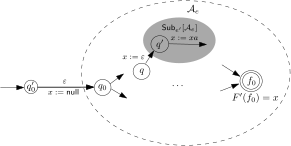
\includegraphics[width = 0.6\textwidth]{psst-extract.pdf}
%\caption{The PSST for $\extract_{i,e}$}
%\label{fig-psst-extract}
%\end{figure}
%\qed
%\end{proof}
%
%
%\begin{proof}[Lemma~\ref{lem-replace}]
%%\paragraph*{Construction of $\cT_{\replaceall_{\pat, \rep}}$.} 
%Let $\$i_1, \cdots, \$i_k$ with $i_1 < \cdots < i_k$ be an enumeration of all the references in $\rep$. 
%Moreover, for every $j \in [k]$, let $e'_{i_j}$ be the subexpression of $\pat$ corresponding to the $i_j$-th capturing group.
%
%Suppose $\cA_\pat = (Q, \Sigma, \delta, \tau, q_0, f_0)$. Then $\cT_{\replace_{\pat,\rep}}$ is obtained from $\cA_\pat$ by adding a fresh states $q'_0$ such that (see Figure~\ref{fig-psst-replace})
%\begin{itemize}
%\item $\cT_{\replace_{\pat,\rep}}$ goes from $q'_0$ to $q_0$ via an $\varepsilon$-transition of higher priority than the non-$\varepsilon$-transitions, in order to search the first match of $\pat$ starting from the current position, 
%%
%\item when $\cT_{\replace_{\pat,\rep}}$ stays at $q'_0$, it keeps appending the current letter to the end of $x_0$, 
%%
%\item starting from $q_0$, $\cT_{\replace_{\pat,\rep}}$ simulates $\cA_\pat$ and stores the matches of the $\$i_1$-th, $\ldots$, $\$i_k$-th capturing groups of $\pat$ into the string variables $x_1, \cdots, x_k$ respectively,   
%%
%\item when the first match of $\pat$ is found, $\cT_{\replace_{\pat,\rep}}$ goes from $f_0$ to $q'_0$ via an $\varepsilon$-transition, appends the replacement string, which is $\rep[x_1/\$_{i_1}, \cdots, x_k/\$_{i_k}]$, to the end of $x_0$, and keeps searching for the next match of $\pat$.
%\end{itemize}
%
%\begin{figure}[ht]
%\centering
%%\rule{\linewidth}{0cm}
%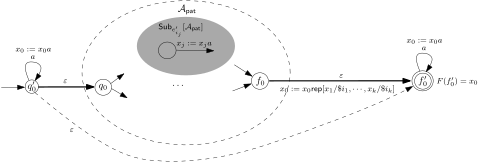
\includegraphics[scale=0.8]{psst-replace.pdf}
%\caption{The PSST for $\replace_{\pat,\rep}$}
%\label{fig-psst-replace}
%\end{figure}
%
%Formally, $\cT_{\replaceall_{\pat, \rep}} =$ $(Q \cup \{q'_0\}$, $\Sigma$, $X$, $\delta'$, $\tau', E, q'_0, F)$ where
%\begin{itemize}
%\item $q'_0 \not \in Q$,
%
%\item  $X = \{x_0, x_1, \cdots, x_k\}$,
%%
%\item $F(q'_0) = x_0$, and $F(q')$ is undefined for every $q' \in Q$,
%%
%\item $\delta'$ and $\tau'$ are obtained from $\delta$ and $\tau$ as follows,
%\begin{itemize}
%\item $\delta'(q'_0, \sigma) = (q'_0)$ for every $\sigma \in \Sigma$, and $\tau'(q'_0) = ((q_0); ())$,
%%
%\item for every $q \in Q \setminus \{f_0\}$ and $\sigma \in \Sigma$, $\delta'(q, \sigma) = \delta(q, \sigma)$ and $\tau'(q) = \tau(q)$, 
%%
%\item $\delta'(f_0, \sigma) = ()$ for every $\sigma \in \Sigma$ and $\tau'(f_0) = ((q'_0); ())$,
%\end{itemize}
%%
%\item $E$ is defined as follows, 
%\begin{itemize}
%\item for every transition $(q, \sigma, q')$ with $\sigma \in \Sigma^\varepsilon$ in $\cA_\pat$, $E(q, \sigma, q')(x_0) = x_0$,
%%
%\item for every transition $(q, \sigma, q')$ with $\sigma \in \Sigma^\varepsilon$ and $j \in [k]$,  if $(q, \sigma, q')$ occurs in ${\sf Sub}_{e'_{i_j}}[\cA_\pat]$, then $E(q, \sigma, q')(x_j) = x_j\sigma$, otherwise, $E(q, \sigma, q')(x_j) = x_j$,
%%
%%\item for all the other transitions $(q, \sigma, q')$ with $\sigma \in \Sigma^\varepsilon$ in $\cA_e$, we have $E(q, \sigma, q')(x) = x$, 
%%
%\item  for every $\sigma \in \Sigma$ and $j \in [k]$, $E(q'_0, \sigma, q'_0)(x_0) = x_0\sigma$ and $E(q'_0, \sigma, q'_0)$$(x_j) = x_j$, 
%
%\item $E(q'_0, \varepsilon, q_0)(x_j) = x_j$ for every $j \in [k] \cup \{0\}$, 
%%
%\item $E(f_0, \varepsilon, q'_0)(x_0) = x_0 \rep[x_1/\$i_1,\ldots, x_k/\$i_k]$, and for every $j \in [k]$, we have $E(f_0, \varepsilon, q'_0)(x_j) = \varepsilon$.
%
%\end{itemize}
%%
%\end{itemize}
%\qed
%\end{proof}

In the rest of this section, we are going to illustrate how to prove Lemma~\ref{lem:psst_preimage}, namely, how to compute the pre-images of regular languages under PSSTs.

\subsection{Computing the pre-image of regular languages under PSSTs}\label{sec-pre-image}

%In this subsection, we are going to show Lemma~\ref{lem:psst_preimage}, namely, how to compute the pre-images of regular languages under PSSTs.

%\tl{another way is to first define B as a PFA, could make the construction a bit modular?}\zhilin{Add a counter example for this natural idea.}
 
Let $\psst = (Q_T, \Sigma$, $X, \delta_T, \tau_T, E_T,  q_{0, T}, F_T)$ be a PSST  and $\Aut
  = (Q_A, \Sigma$, $\delta_A$, $q_{0, A}$, $F_A)$ be an \FA{}. Without loss of generality, we assume that $\Aut$ contains no $\varepsilon$-transitions. For convenience, we use $\cE(\tau_T)$ to denote $\{(q, q') \mid q' \in \tau_T(q)\}$. 

To illustrate the intuition of the proof of Lemma~\ref{lem:psst_preimage}, let us start with the following natural idea of firstly constructing a PFA $\cB$ for the pre-image: $\cB$ simulates a run of $\psst$ on $w$, and, for each $x \in X$, records an $\Aut$-abstraction of the string stored in $x$, that is, the set of state pairs $(p, q) \in Q_A \times Q_A$ such that starting from $p$, $\Aut$ can reach $q$ after reading the string stored in $x$. Specifically, the states of $\cB$ are of the form $(q, \rho)$ with $q \in Q$ and $\rho \in (\cP(Q_A \times Q_A ))^{X}$. Moreover, the priorities of $\cB$ inherit those of $\psst$. The PFA $\cB$ is then transformed to an equivalent FA by simply dropping all priorities. We refer to this FA as $\cB'$.

Nevertheless, it turns out that this construction is flawed: A string $w$ is in $\cR^{-1}_{\cT}(\Lang(\Aut))$ iff the (unique) accepting run of $\cT$ on $w$ produces an output $w'$ that is accepted by $\Aut$. However, a string $w$ is accepted by $\cB'$ iff \emph{there is a run of $\cT$ on $w$, not necessarily of the highest priority}, producing an output $w'$ that is accepted by $\Aut$. The following example illustrates the flaw of the construction above.

\begin{example}
\label{pre-image-count-examp}
Let $\cT_{\tt extract_{decimalReg,1}}$ be the PSST in Fig.~\ref{fig-psst-exmp} and $\cA$ be the FA corresponding to the regular expression $\{1,\cdots,9\}^*$, specifically, $\cA= (\{p_0\}$, $\{0,\cdots,9\}$, $\delta_A$, $p_0, \{p_0\})$, where $\delta_A = \{(q_0, \ell, q_0) \mid \ell = 1, \cdots, 9\}$.
%  in Figure~\ref{fig-pre-image-count-exmp}, that is, 
%\begin{itemize}
%\item $\cT=(\{q_0, q_1, q_2\}, \{a,b,c\}, \{x_0\}, \delta_T, \tau_T, E_T, q_0, F_T)$, where $\delta_T(q_0, \sigma) = (q_0)$, $\delta_T(q_1, a) = (q_1)$, $\delta_T(q_2, \sigma) = (q_2)$, $\tau_T(q_0) = ((q_1); ())$, $\tau_T(q_1)=((q_0, q_2);())$, and $\tau_T(q_2)= ((); ())$, $E_T(q_0, \sigma, q_0) (x_0) = x_0 \sigma$, $E_T(q_1, \varepsilon, q_0) (x_0) = x_0 c$, $E_T(q_1, \varepsilon, q_2) (x_0) = x_0 c$, $E_T(q_2, \sigma, q_2) (x_0) = x_0 \sigma$, for $\sigma \in\{ a, b\}$. Moreover, $F_T(q_2)= x_0$;
%
%\item $\cA = (\{p_0\}, \{a,b,c\}, \delta_A, p_0, \{p_0\})$, where $\delta_A$ = $\{(p_0, \sigma, p_0)$ $\mid \sigma = b, c\}$.
%\end{itemize}

Let us consider $w = 10$. The accepting run of $\cT_{\tt extract_{decimalReg,1}}$ on $w$ is $q_0 \xrightarrow[x_1:=x_11]{1} q_1 \xrightarrow[x_1:=x_10]{0} q_1 \xrightarrow{\varepsilon} q_2 \xrightarrow{\varepsilon} q_3 \xrightarrow{\varepsilon} q_4 \xrightarrow{\varepsilon} q_5 \xrightarrow{\varepsilon} q_6$, producing an output $10 \not \in \Lang(\cA)$. Therefore, $10 \not \in \cR_\cT^{-1}(\Lang(\cA))$. Nevertheless, if we consider the FA $\cB'$ constructed from $\cT$ and $\cA$,  it turns out that $\cB'$ does accept $w$, witnessed by the run $(q_0, \{(p_0,p_0)\}) \xrightarrow{1} (q_1, \{(p_0, p_0)\}) \xrightarrow{\varepsilon} (q_2, \{(p_0, p_0)\}) \xrightarrow{\varepsilon}  (q_3, \{(p_0, p_0)\}) \xrightarrow{\varepsilon}  (q_4, \{(p_0, p_0)\}) \xrightarrow{\varepsilon}  (q_5, \{(p_0, p_0)\}) \xrightarrow{0}  (q_5, \{(p_0, p_0)\}) \xrightarrow{\varepsilon}  (q_6, \{(p_0, p_0)\})$, where $\{(p_0, p_0)\}$ is the $\cA$-abstraction of the strings $\varepsilon$ and $1$. On the other hand, the run of $\cB'$ corresponding to the accepting run of $\cT$ on $w$, i.e. $(q_0, \{(p_0, p_0)\}) \xrightarrow{1} (q_1, \{(p_0, p_0)\}) \xrightarrow{0} (q_1, \emptyset) \xrightarrow{\varepsilon}  (q_2, \emptyset) \xrightarrow{\varepsilon} (q_3, \emptyset) \xrightarrow{\varepsilon} (q_4, \emptyset) \xrightarrow{\varepsilon} (q_5, \emptyset) \xrightarrow{\varepsilon} (q_6, \emptyset)$, is not accepting, where $\{(p_0,p_0)\}$ is the $\cA$-abstraction of $\varepsilon$ as well as $1$, and $\emptyset$ is the $\cA$-abstraction of $10$.
\end{example}

%%%%%%%%%%%%%%%%%%%%%%%%%%%%%%
%%%%%%%%%%%%%%%%%%%%%%%%%%%%%%
\hide{
\begin{example}
\label{pre-image-count-examp}
Let $\cT$ be the PSST and $\cA$ be the FA in Figure~\ref{fig-pre-image-count-exmp}, that is, 
\begin{itemize}
\item $\cT=(\{q_0, q_1, q_2\}, \{a,b,c\}, \{x_0\}, \delta_T, \tau_T, E_T, q_0, F_T)$, where $\delta_T(q_0, \sigma) = (q_0)$, $\delta_T(q_1, a) = (q_1)$, $\delta_T(q_2, \sigma) = (q_2)$, $\tau_T(q_0) = ((q_1); ())$, $\tau_T(q_1)=((q_0, q_2);())$, and $\tau_T(q_2)= ((); ())$, $E_T(q_0, \sigma, q_0) (x_0) = x_0 \sigma$, $E_T(q_1, \varepsilon, q_0) (x_0) = x_0 c$, $E_T(q_1, \varepsilon, q_2) (x_0) = x_0 c$, $E_T(q_2, \sigma, q_2) (x_0) = x_0 \sigma$, for $\sigma \in\{ a, b\}$. Moreover, $F_T(q_2)= x_0$;
%
\item $\cA = (\{p_0\}, \{a,b,c\}, \delta_A, p_0, \{p_0\})$, where $\delta_A$ = $\{(p_0, \sigma, p_0)$ $\mid \sigma = b, c\}$.
\end{itemize}

Let us consider $w = a$. The accepting run of $\cT$ on $w$ is $q_0 \xrightarrow{\varepsilon} q_1 \xrightarrow[x_0:=x_0c]{\varepsilon} q_0 \xrightarrow[x_0:=x_0a]{a} q_0 \xrightarrow{\varepsilon} q_1 \xrightarrow[x_0:=x_0c]{\varepsilon} q_2$, producing an output $cac \not \in \Lang(\cA)$. Therefore, $a \not \in \cR_\cT^{-1}(\Lang(\cA))$. Nevertheless, if we consider the FA $\cB'$ constructed from $\cT$ and $\cA$,  it turns out that $\cB'$ does accept $w$, witnessed by the run $(q_0, \{(p_0,p_0)\}) \xrightarrow{\varepsilon} (q_1, \{(p_0,p_0)\}) \xrightarrow{a} (q_1, \{(p_0, p_0)\}) \xrightarrow{\varepsilon}  (q_2, \{(p_0, p_0)\})$. On the other hand, the run of $\cB'$ corresponding to the accepting run of $\cT$ on $w$, i.e. $(q_0, \{(p_0,p_0)\}) \xrightarrow{\varepsilon} (q_1, \{(p_0,p_0)\}) \xrightarrow{\varepsilon} (q_0, \{(p_0, p_0)\}) \xrightarrow{a}  (q_0, \emptyset) \xrightarrow{\varepsilon} (q_1, \emptyset) \xrightarrow{\varepsilon} (q_2, \emptyset)$, is not accepting, where $\{(p_0,p_0)\}$ and $\emptyset$ are the $\cA$-abstractions of $x_0$.
\end{example}

\begin{figure}[ht]
\centering
%\rule{\linewidth}{0cm}
\includegraphics[scale=0.8]{pre-image-counter-example.pdf}
\caption{A counterexample to disprove the flawed pre-image construction method}
\label{fig-pre-image-count-exmp}
\end{figure}
}
%%%%%%%%%%%%%%%%%%%%%%%%%%%%%%%%
%%%%%%%%%%%%%%%%%%%%%%%%%%%%%%%%

%\begin{proof}[Lemma~\ref{lem:psst_preimage}]

%We are ready to prove Lemma~\ref{lem:psst_preimage}.

%Let $\psst = (Q_T, \Sigma$, $X, \delta_T, \tau_T, E_T,  q_{0, T}, F_T)$ be a PSST and $\Aut= (Q_A, \Sigma, \delta_A, q_{0, A}, F_A)$ be an \FA{}. 
While the aforementioned natural idea does not work,  we choose to construct an FA $\cB$ that simulates the \emph{accepting} run of $\psst$ on $w$, and, for each $x \in X$, records an $\Aut$-abstraction of the string stored in $x$, that is, the set of state pairs $(p, q) \in Q_A \times Q_A$ such that starting from $p$, $\Aut$ can reach $q$ after reading the string stored in $x$. 
To simulate the accepting run of $\psst$, it is necessary to record all the states accessible through the runs of higher priorities to ensure the current run is indeed the accepting run of $\psst$ (of highest priority). Moreover, $\cB$ also remembers the set of $\varepsilon$-transitions of $\cT$ after the latest non-$\varepsilon$-transition to ensure that no transition occurs twice in a sequence of $\varepsilon$-transitions of $\cT$.

Specifically, each state of $\cB$ is of the form $(q, \rho, \Lambda, S)$, where $q \in Q_T$, $\rho \in (\cP(Q_A \times Q_A ))^{X}$, $\Lambda \subseteq \cE(\tau_T)$, and $S \subseteq Q_T$. 
For a state $(q, \rho, \Lambda, S)$, our intention for $S$ is that the states in it are those that can be reached in the runs of higher priorities than the current run, by reading the same sequence of letters and applying the $\varepsilon$-transitions as many as possible. Note that when recording in $S$ all the states accessible through the runs of higher priorities, we do not take the non-repetition of $\varepsilon$-transitions into consideration since if a state is reachable by a sequence of $\varepsilon$-transitions where some $\varepsilon$-transitions are repeated, then there exists also a sequence of non-repeated $\varepsilon$-transitions reaching the state. 
Moreover, when simulating an $a$-transition of $\cT$ (where $a \in \Sigma$) at a state $(q, \rho, \Lambda, S)$, suppose $\delta_T(q, a) = (q_1, \cdots, q_m)$ and $\tau_T(q) = (P_1, P_2)$, then $\cB$ nondeterministically chooses $q_i$ and goes to the state $(q_i, \rho', \emptyset, S')$, where 
\begin{itemize}
\item $\rho'$ is obtained from $\rho$ and $E_T(q, \sigma, q_i)$, 
%
\item $\Lambda$ is reset to $\emptyset$,
% 
\item all the states obtained from $S$ by applying  an $a$ transition should be \emph{saturated by $\varepsilon$-transitions} and put into $S'$, more precisely, all the states reachable from $S$ by first applying an $a$-transition, then a sequence of $\varepsilon$-transitions, should be put into $S'$,
%
\item moreover, all the states obtained from $q_1,\cdots, q_{i-1}$ (which are of higher priorities than $q_i$) by saturating with $\varepsilon$-transitions should be put into $S'$,
%
\item finally, all the states obtained from those in $P'_1 = \{q' \in P_1 \mid (q, q') \not \in \Lambda\}$ (which are of higher priorities than $q_i$) by saturating with non-$\Lambda$ $\varepsilon$-transitions first (i.e. the $\varepsilon$-transitions that do not belong to $\Lambda$), and applying an $a$-transition next, finally saturating with $\varepsilon$-transitions again, should be put into $S'$, (note that according to the semantics of PSST, the $\varepsilon$-transitions in $\Lambda$ should be avoided when defining $P'_1$ and saturating the states in $P'_1$ with $\varepsilon$-transitions). 
\end{itemize}
%For technical reasons, when constructing $\cB$, we assume that this saturation happens when a state is added to $S$ for the first time. Therefore, at a state $(q, \rho, \Lambda, S)$, all the states reachable from the states in $S$ by sequences of $\varepsilon$-transitions in $\cT$ have already been in $S$.

The above construction  does not utilize the so-called \tmtextit{copyless} property (i.e. for each transition $t$ and each variable $x$, $x$ appears at most once on the right-hand side of the assignment for $t$) \cite{AC10,AD11}, 
  thus it works for general, or \textit{copyful}, PSSTs \cite{FR17}.

The formal construction of $\cB$ is omitted, due to the page limit. The interested readers can read Appendix~\ref{app-pre-image} for more details.

%%%%%%%%%%%%%%%%%%%%%%%%%%%%%%%%%%%
%%%%%%%%%%%%%%%%%%%%%%%%%%%%%%%%%%%
\hide{
\begin{table}[t]
\centering
\caption{the actual $\cB$ state in Figure 
\label{table:psst-preimage}
\ref{fig-psst-preimage-exmp}}
\begin{tabular}{|c|c|}
    \hline
    Symbol & State of $\cB$\\
    \hline
    $r_0$ & $(q_0, \rho_1, \emptyset, \emptyset)$\\
    \hline
    $r_1$ & $(q_1, \rho_1, \{ (q_0, q_1) \}, \emptyset)$\\
    \hline
    $r_2$ & $(q_2, \rho_1, \{ (q_0, q_1), (q_1, q_2) \}, \{ q_0 \})$\\
    \hline
    $r_3$ & $(q_2, \rho_2, \emptyset, \{ q_0, q_1, q_2 \})$\\
    \hline
    $r_4$ & $(q_2, \rho_1, \emptyset, \{ q_0, q_1, q_2 \})$\\
    \hline
    $r_5$ & $(q_0, \rho_1, \{ (q_0, q_1) (q_1, q_0) \}, \emptyset)$\\
    \hline
    $r_6$ & $(q_0, \rho_2, \emptyset, \emptyset)$\\
    \hline
    $r_7$ & $(q_0, \rho_2, \emptyset, \{ q_0, q_1, q_2 \})$\\
    \hline
    $r_8$ & $(q_1, \rho_2, \{ (q_0, q_1) \}, \{ q_0, q_1, q_2 \})$\\
    \hline
    $r_9$ & $(q_0, \rho_2, \{ (q_0, q_1) (q_1, q_0) \}, \{ q_0, q_1, q_2 \})$\\
    \hline
    $r_{10}$ & $(q_2, \rho_2, \{ (q_0, q_1) (q_1, q_2) \}, \{ q_0, q_1, q_2 \})$\\
    \hline
    $r_{11}$ & $(q_0, \rho_1, \emptyset, \{ q_0, q_1, q_2 \})$\\
    \hline
    $r_{12}$ & $(q_1, \rho_1, \{ (q_0, q_1) \}, \{ q_0, q_1, q_2 \})$\\
    \hline
    $r_{13}$ & $(q_0, \rho_1, \{ (q_0, q_1) (q_1, q_0) \}, \{ q_0, q_1, q_2 \})$\\
    \hline
    $r_{14}$ & $(q_2, \rho_1, \{ (q_0, q_1) (q_1, q_2) \}, \{ q_0, q_1, q_2 \})$\\
    \hline
    $r_{15}$ & $(q_2, \rho_2, \{ (q_0, q_1) (q_1, q_2) \}, \{ q_0 \})$\\
    \hline
    $r_{16}$ & $(q_1, \rho_2, \emptyset, \{ q_0, q_1, q_2 \})$\\
    \hline
    $r_{17}$ & $(q_2, \rho_2, \{ (q_1, q_2) \}, \{ q_0, q_1, q_2 \})$\\
    \hline
    $r_{18}$ & $(q_0, \rho_2, \{ (q_1, q_0) \}, \{ q_0, q_1, q_2 \})$\\
    \hline
    $r_{19}$ & $(q_1, \rho_2, \{ (q_1, q_0) (q_0, q_1) \}, \{ q_0, q_1, q_2 \})$\\
    \hline
    $r_{20}$ & $(q_2, \rho_2, \{ (q_1, q_0) (q_0, q_1) (q_1, q_2) \}, \{ q_0, q_1, q_2 \})$\\
    \hline
    $r_{21}$ & $(q_1, \rho_2, \{ (q_0, q_1) \}, \emptyset)$\\
    \hline
    $r_{22}$ & $(q_0, \rho_2, \{ (q_0, q_1) (q_1, q_0) \}, \emptyset)$\\
    \hline
\end{tabular}
\end{table}
}
%%%%%%%%%%%%%%%%%%%%%%%%%%%%%%%%%%%
%%%%%%%%%%%%%%%%%%%%%%%%%%%%%%%%%%%

%
%\zhilin{stopped here}
%\zhilei{changed a little bit}

%%%%%%%%%%%%%%%%%%%%%%%%%%%%%%%%%%%%%%%%%
%%%%%%%%%%%%%%%%%%%%%%%%%%%%%%%%%%%%%%%%%
\hide{
\subsection{Complexity}

\begin{proposition}[POPL'19]
	The path feasibility problem of the following two fragments is non-elementary: SL with 2FTs, and SL with FTs+replaceAll.
	
	SL[conc, replaceAll, reverse, FFT] is expspace-complete (note that 2FTs in SL are restricted to be one-way and functional)
\end{proposition}

%The same proof strategy can be used for FTs+replaceAll. The 2FTs used in the proof above
%proceed by running completely over the word and producing some output, then silently moving
%back to the beginning of the word. An arbitrary number of passes are made in this way. We
%can simulate this behaviour using FTs and replaceAll.


The main open question is the complexity of the SL fragment with replaceall function and prioritized streaming transducers. Note that PSST can simulate 2FT (adapting Matt's proof?), so we could obtain nonelementary lower bound for SL with PSST.

However, this variant of replaceall is quite different from the replaceall we had before ...

\begin{enumerate}
\item  does  copyless help?
\item how about SL with only this version of replaceall?
\end{enumerate}
}
%%%%%%%%%%%%%%%%%%%%%%%%%%%%%%%%%%%%%%%%%
%%%%%%%%%%%%%%%%%%%%%%%%%%%%%%%%%%%%%%%%%


%%%%%%%%%%%%%%%%%%%%%%%%%%%%

\section{Implementation and Experiments}
\label{sect:impl}

We have implemented our decision procedure for $\strline$ in the SMT solver OSTRICH \cite{CHL+19}, which provides a modular and easy-to-use framework for extending all sorts of string operations. As shown in \ref{sec:decision}, \PSST s satisfy the conditions required by the backwards reasoning approach of OSTRICH, which enables us to integrate our logic with standard string theory.

Our implementation supports three operators


%%%%%%%%%%%%%%%%%%%%%%%%%%%%
%\input{experiments.tex}

%%%%%%%%%%%%%%%%%%%%%%%%%%%%

\bibliographystyle{alpha}
\bibliography{string}

\newpage
%% Appendix
\appendix

%!TEX root = popl2018.tex

\appendix

\begin{center}
{\huge Supplementary Material} \\
{\large ``What's Decidable About String Constraints with ReplaceAll Function?''} 
\end{center}

\bigskip

We provide below proofs and examples that were omitted from the main text due to space constraints.

%%%%%%%%%%%%%%%%%%%%%%%%%%%%%%%%%%%%%%%%%%%%%%%%%%%%%%%%%
%%%%%%%%%%%%%%%%%%%%%%%%%%%%%%%%%%%%%%%%%%%%%%%%%%%%%%%%%
\hide{
\noindent {\it Proposition~\ref{prop-num-path}}.
{\it Let $G=(V,E)$ be a DAG such that the out-degree of each vertex is at most two. Then there are $n^{O(\dmdidx(G))}$ different paths  in $G$.
}

\begin{proof}
\end{proof}
}
%%%%%%%%%%%%%%%%%%%%%%%%%%%%%%%%%%%%%%%%%%%%%%%%%%%%%%%%%
%%%%%%%%%%%%%%%%%%%%%%%%%%%%%%%%%%%%%%%%%%%%%%%%%%%%%%%%%
\def\refpropundpat{\ref{prop-und-pat-var}}

\section{Proof of Proposition~\protect\refpropundpat}
\label{sec:prop-und-pat-var-proof}

We recall Proposition~\ref{prop-und-pat-var} and then give its proof.

\medskip

\noindent \textsc{Proposition}~\ref{prop-und-pat-var}
{\em The satisfiability problem of $\strline[\replaceall]$ is undecidable, if the second parameters of the $\replaceall$ terms are allowed to be variables.
}

\begin{proof}
	We reduce from the Post Correspondence Problem (PCP). Recall that the input of the problem consists of two finite lists $\alpha_{1},\ldots ,\alpha_{N}$ and $\beta_1,\ldots ,\beta_N$ of nonempty strings over $\Sigma$. A solution to this problem is a sequence of indices $(i_{k})_{1\leq k\leq K}$ with $ K\geq 1$ and $ 1\leq i_{k}\leq N$ for all $k$, such that
	$	\alpha _{{i_{1}}}\ldots \alpha _{{i_{K}}}=\beta _{{i_{1}}}\ldots \beta _{{i_{K}}}.
	$
	The PCP problem is to decide whether such a solution exists or not.
	
	Without loss of generality, suppose $\Sigma \cap [N] = \emptyset$ and $\$ \not \in \Sigma \cup [N]$. Let $\Sigma' = \Sigma \cup [N] \cup \{\$\}$. We will construct an $\strline[\replaceall]$ formula $C$ over $\Sigma'$ such that the PCP instance has a solution iff $C$ is satisfiable. To this end, the formula $C$ utilises the capability that the second parameter of the $\replaceall$ terms may be variables.
	
	Let $x_1, \cdots, x_N, y_1, \cdots, y_N, z$ be mutually distinct string variables. Then the formula $C = \varphi \wedge \psi$, where 
	%
	$$
	\begin{array}{l c l}
	\varphi & = & \bigwedge \limits_{i \in [N]} (x_i = \replaceall(x_{i-1}, i, \alpha_i) \wedge y_i = \replaceall(y_{i-1}, i, \beta_i)) \wedge  z = \replaceall(x_N, y_N, \$), \\
	\psi & = & x_0 \in (1 + \cdots + N)^+ \wedge z \in \$.
	\end{array}
	$$
	
	It is not hard to see that $\varphi$ is a straight-line relational constraint, thus $C$ is an $\strline[\replaceall]$ formula. Note that in $\replaceall(x_N, y_N, \$)$, the second parameter is a variable. We show that $C$ is satisfiable iff the PCP instance has a solution: $C$ is satisfiable iff there is a string $i_1 \cdots i_K \in \Ll((1 + \cdots + N)^+)$ such that when $x_0$ is assigned with $i_1 \cdots i_K$, the value of $z$ is $\$$.
	Since $z = \replaceall(x_N, y_N, \$)$ and $x_N, y_N \in \Sigma^+$, we know that $z$ is $\$$ iff the values of $x_N$ and $y_N$ are the same. Therefore, $C$ is satisfiable iff there is a string $i_1 \cdots i_K \in \Ll((1 + \cdots + N)^+)$ such that when $x_0$ is assigned with $i_1 \cdots i_K$, the values of $x_N$ and $y_N$ are the same. Therefore, $C$ is satisfiable iff there is a sequence of indices $i_1 \cdots i_K$ such that $\alpha_{i_1} \cdots \alpha_{i_K} = \beta_{i_1} \cdots \beta_{i_K}$, that is, the PCP instance has a solution.
	%
	%
	%Suppose the PCP instance has a solution. Then there is a sequence of indices $i_1 \cdots i_K$ such that $\alpha _{{i_{1}}}\ldots \alpha _{{i_{K}}}=\beta _{{i_{1}}}\ldots \beta _{{i_{K}}}$. Let $x_0$ be $i_1 \cdots i_K$. Then from the construction of $C$, we know that the values of $x_N$ and $y_N$ are $\alpha _{{i_{1}}}\ldots \alpha _{{i_{K}}}$ and  $\beta _{{i_{1}}}\ldots \beta _{{i_{K}}}$ respectively. Thus the values of $x_N$ and $y_N$ are the same. Therefore, the value of $z=\replaceall(x_N, y_N, \$)$ is $\$$. The formula $C$ is satisfiable. 
	%
	%
	%Since $x_0 \in (1 + \cdots + N)^+$, we know that $x_N, y_N$ can only be strings over the alphabet $\Sigma$. Therefore, $z \in \$$ iff $x_N = y_N$.
	%
	%	
	%	We then introduce, for $i=1,\cdots, N$, 
	%	$x_{i+1}=\replaceall(x_0, \alpha_i, i)$ and $y_{i+1}=\replaceall(y_0, \beta_i, i)$, 
	%	$x_0'=\replaceall(x_0, \sharp, \epsilon)$ and $y_0'=\replaceall(y_0, \sharp, \epsilon)$
	%	
	%	$x_{N+1}=y_{N+1}$, $x_0'=y'_0$
	%	
	%	
	%	with regular constraints $x_0\in \sharp((\sum_{i=1}^N\alpha_i)\sharp)^*$ and $y_0\in \sharp((\sum_{i=1}^N\beta_i)\sharp)^*$,
	%	
	%	where $z=z'$ can be encoded by 
	%		$z''=\replaceall(z, z', \$)$ and $z''\in \$$. 
\end{proof}

\def\refsecreplaceallsl{\ref{sec:replaceallsl}}

\section{Section~\protect\refsecreplaceallsl: The Correctness of the decision procedure}
\label{sec:dp-sl-correctness}

We argue that the procedure in Section~\ref{sec:dp-sl-general} is correct.
Note that Proposition~\ref{prop-sat-sl-case} removed a single $\replaceall(-,-,-)$ to obtain only regular constraints.
Each step of our decision procedure effectively eliminates a $\replaceall(-,-,-)$.
Similar to Proposition~\ref{prop-sat-sl-case}, each step maintains the satisfiability from the preceding step.

In more detail, from each $G_i$ we can define a constraint $C_i$. This constraint is a conjunction of the following atomic constraints.
\begin{itemize}
\item For each variable $x$ such that $(x, (\rpleft, a), y)$ and $(x, (\rpright,a), z)$ are the edges in $G_i$, we assert in $C_i$ that $x = \replaceall(y, a, z)$.
\item In addition, for each variable $x$ such that $\cE_i(x)$ is not empty, moreover, \emph{either $x$ is a source variable in $G_C$ (not $G_i$) or there are (incoming or outgoing) edges connected to $x$ in $G_i$}, let $e_i(x)$ be the regular expression equivalent to the conjunction of all constraints in $\cE_i(x)$ (Note that the conjunction of multiple regular expressions still defines a regular language). We assert in $C_i$ that $x \in e_i(x)$. Note that if $x$ is not a source variable in $G_C$ and there are no edges connected to $x$ in $G_i$, then the regular constraints in $\cE_i(x)$ are not included into $C_i$.
\end{itemize}

%This constraint is a conjunction of the following clauses.
%For each variable $x$ such that $\cE_i(x)$ is not empty, we let $e_i(x)$ be the regular expression equivalent to the conjunction of all constraints in $\cE_i(x)$.
%Since this is the conjunction of multiple regular expressions (NFAs), it is regular.
%We assert in $C_i$ that $x \in e_i(x)$.

It is immediate that $C_0$ is equivalent to $C$.
We require the following proposition, which gives us the correctness of the decision procedure by induction.
Note that the final $C_i$ when exiting the loop will be a conjunction of regular constraints on the source variables.

\begin{proposition}
    For each $i$,  let the $\rpleft$-edge and the $\rpright$-edge from $x$ to $y$ and $z$ respectively be the two edges removed from $G_i$ to construct $G_{i+1}$. Then $C_i$ is satisfiable iff there are sets $T_{j, z}$ such that $C_{i+1}$ is satisfiable.
\end{proposition}

We can see the above proposition by observing that, in each step, $C_i$ is of the form
\[
    x = \replaceall(y, a, z) \wedge x \in e_i(x) \wedge y \in e_i(y) \wedge z \in e_i(z) \wedge C'
\]
where $C'$ does not contain $x$, and $C_{i+1}$ is of the form
\[
    y \in e_{i+1}(y) \wedge z \in e_{i+1}(z) \wedge C' \ .
\]
Note that $C'$ remains unchanged since only the two edges leaving $x$ are removed from $G_i$ and $\cE_{i+1}(x') = \cE_i(x')$ for all $x'$ distinct from $x$, $y$, and $z$.
First assume $y \neq z$.
Supposing $C_i$ is satisfiable, an argument similar to that of Proposition~\ref{prop-sat-sl-case} shows that there are sets $T_{j,z}$ such that the same values of $y$ and $z$ also satisfy $e_{i+1}(y)$ and $e_{i+1}(z)$.
Since $C'$ is unchanged, all $x'$ distinct from $x$, $y$, and $z$ can also keep the same value.
Thus, $C_{i+1}$ is also satisfiable.
In the other direction, suppose that there are sets $T_{j, z}$ such that $C_{i+1}$ is satisfiable. Take a satisfying assignment to $C_{i+1}$.
From the assignment to $y$ and $z$ we obtain as in Proposition~\ref{prop-sat-sl-case} an assignment to $x$ that satisfies $\replaceall(y, a, z) \wedge x \in e_i(x)$.
Furthermore, the assignments for $y$ and $z$ also satisfy $e_i(y)$ and $e_i(z)$ since $\cE_i(y)$ and $\cE_i(z)$ are subsets of $\cE_{i+1}(y)$ and $\cE_{i+1}(z)$.
Finally, since $C'$ is unchanged, the assignments to all other variables also transfer, giving us a satisfying assignment to $C_i$ as required.
In the case where $y = z$, the arguments proceed analogously to the case $y \neq z$.

\def\prodauttitle{$\cA_1 \times \cA_u$}
\def\defutitle{$u = 010$}
\section{The product automaton \protect\prodauttitle for \protect\defutitle}

In Figure~\ref{fig-cs-exmp} we give the product automaton $\cA_1 \times \cA_u$ for $u = 010$.
This is a straightforward product construction, but may be useful for reference when understanding Figure~\ref{fig-cs-exmp-2} which shows the automaton $\cB_{\cA_1, u, T_z}$ which is derived from the product.

\begin{figure}[htbp]
\begin{center}
\includegraphics[scale=0.65]{constant-string-example.pdf}
\end{center}
\caption{The NFA $\cA_1 \times \cA_u$ for $u = 010$}\label{fig-cs-exmp}
\end{figure}
%

\def\refsecreplaceallcs{\ref{sec:replaceallcs}}
\section{Complexity analysis in Section~\protect\refsecreplaceallcs}
\label{sec:cs-complexity-full}

We provide a more detailed analysis of the complexity of the algorithm for the constant string case, described in Section~\ref{sec:replaceallcs}.
A summary of this argument already appears in Section~\ref{sec:replaceallcs}.

When constructing $G_{i+1}$ from $G_i$, suppose the two edges from $x$ to $y$ and $z$ respectively are currently removed, let the labels of the two edges be $({\sf l}, u)$ and $({\sf r}, u)$ respectively, then each element $(\cT, \cP)$ of $\cE_i(x)$ may be transformed into an element $(\cT', \cP')$ of $\cE_{i+1}(y)$ such that $|\cT'| = O(|u||\cT|)$, meanwhile, it may also be transformed into an element $(\cT'', \cP'')$ of $\cE_{i+1}(z)$ such that $\cT''$ has the same state space as $\cT$. Thus, for each source variable $x$, $\cE(x)$ contains at most exponentially many elements, and each of them may have a state space of at most exponential size. For instance, for a path from $x'$ to $x$ where the constant strings $u_1,\cdots, u_n$ occur in the labels of edges, an element $(\cT,\cP) \in \cE_0(x')$ may induce an element $(\cT', \cP')$ of $\cE(x)$ such that $|\cT'| \le |\cT| |u_1| \cdots |u_n|$, which is exponential in the worst case. 
%
To solve the nonemptiness problem of the intersection of all these regular constraints, the exponential space is sufficient. Consequently, in this case, we still obtain an EXPSPACE upper-bound. 

Let us now consider the special situation that the $\rpleft$-length of $G_C$ is bounded by a constant $c$.
Since $\dmdidx(G_C) \le \lftlen(G_C)$, we know that $\dmdidx(G_C)$ is also bounded by $c$. Therefore, according to Proposition~\ref{prop-di}, there are at most polynomially different paths in $G_C$, we deduce that for each source variable $x$, $\cE(x)$ contains at most polynomially many elements. In addition, since the number of $\rpleft$-edges in each path is bounded by $c$, during the execution of the decision procedure, the number of times when $(\cT, \cP)$ of $\cE_i(x)$ may be transformed into an element $(\cT', \cP')$ of $\cE_{i+1}(y)$ such that $|\cT'| = O(|u||\cT|)$ is bounded by $c$.
Therefore, for each source variable $x$ and each element $(\cT'', \cP'')$ in $\cE(x)$,  $|\cT''|$ is at most polynomial in the size of $C$. We then conclude that for each source variable $x$, $\cE(x)$ corresponds to the intersection of polynomially many regular constraints such that each of them has a state space of polynomial size. Therefore, the nonemptiness of the intersection of all the regular constraints in $\cE(x)$ can be solved in polynomial space. In this situation, we obtain a PSPACE upper-bound.


\def\refsecreplaceallre{\ref{sec:replaceallre}}
\section{Complexity analysis in Section~\protect\refsecreplaceallre}
\label{sec:re-complexity-full}

We provide a more detailed analysis of the complexity of the algorithm for the regular-expression case, described in Section~\ref{sec:replaceallre}.
A summary of this argument already appears in Section~\ref{sec:replaceallre}.

In each step of the reduction, suppose the two edges out of $x$ are currently removed, let the two edges be from $x$ to $y$ and $z$ and labeled by $({\sf l}, e)$ and $({\sf r}, e)$ respectively, then each element of $(\cT, \cP)$ of $\cE_i(x)$ may be transformed into an element $(\cT',\cP')$ of $\cE_{i+1}(y)$ such that $|\cT'| = |\cT| \cdot 2^{O(p(|e|))}$, meanwhile, it may also be transformed into an element $(\cT'',\cP'')$ of $\cE_{i+1}(y)$ such that $\cT''$ has the same state space as $\cT$. Thus, after the reduction, for each source variable $x$, $\cE(x)$ may contain exponentially many elements, and each of them may have a state space of exponential size, more precisely, if we start from a vertex $x$ without predecessors, with an element $(\cT,\cP)$ in $\cE_0(x)$, and go to a source variable $y$ through a path where $k$ edges have been traversed and removed, let $e_1,\cdots, e_k$ be the regular expressions occurring in the labels of these edges, then the resulting element in $\cE(y)$ has a state space of size $|\cT| \cdot 2^{O(p(|e_1|))} \cdot 2^{O(p(|e_2|))} \cdot \cdots \cdot 2^{O(p(|e_k|))}$ in the worst case. To solve the nonemptiness problem of the intersection of all these regular constraints, the exponential space is sufficient. Consequently, for the most general case of regular expressions, we still obtain an EXPSPACE upper-bound. 

On the other hand, for the situation that the $\rpleft$-length of $G_C$ is at most one, we wan to show that the algorithm runs in polynomial space. Suppose the $\rpleft$-length of $G_C$ is at most one. Then the diamond index of $G_C$ is at most one as well. According to Proposition~\ref{prop-di}, there are only polynomially many paths in $G_C$. Nevertheless, for each source variable $x$, $\cE(x)$ may contain an element $(\cT,\cP)$ such that $|\cT|$ is exponential. Since $|\cP|$ may be exponential, $(\cT,\cP)$ may correspond to the intersection of exponentially many regular constraints. However, we can show that $|\cP|$ is at most polynomial, as a result of the fact that the $\rpleft$-length of $G_C$ is at most one. The arguments proceed as follows: Suppose two edges from $x$ to $y, z$ respectively are removed, and an element $(\cT', \cP')$ of $\cE_{i+1}(y)$ such that $|\cT'|$ is exponential and $|\cP'|$ is polynomial, is generated from an element of $(\cT, \cP)$ of $\cE_i(x)$. Then $y$ must be a source variable in $G_C$. Otherwise, there is an $\rpleft$-edge out of $y$ and the $\rpleft$-length of $G_C$ is at least two, a contradiction. Therefore, $y$ is a source variable in $G_C$, $(\cT', \cP')$  will not be used to generate the regular constraints for the other variables. In other words, $y$ is a source variable in $G_C$, and $(\cT', \cP') \in \cE(y)$ with $|\cP'|$ polynomial. We then conclude that for each source variable $x$, $|\cE(x)|$  is at most polynomial in the size of $C$ and for each element $(\cT, \cP) \in \cE(x)$, $|\cP|$ is polynomial in the size of $C$. Therefore, for each source variable $x$,  $\cE(x)$ corresponds to the intersection of polynomially many regular constraints, where each of them has a state space at most exponential size. To solve the nonemptiness of the intersection of these regular constraints, the polynomial space is sufficient. We obtain a PSPACE upper-bound for the situation that the $\rpleft$-length of $G_C$ is at most one.


\def\refsecreplaceallre{\ref{sec:replaceallre}}
\section{Examples in Section~\protect\refsecreplaceallre}

Due to space constraints, we did not provide examples of the decision procedure for the regular-expression case.
We provide some examples here.


\begin{example}\label{exmp-pa-re}
	Let $e_0 = 0^*0 1(1^* + 0^*)$. Then $\cA_{0}$ and $\cA_{e_0}$ are illustrated in Figure~\ref{fig-pa-re}, where ${\sf sleft}$ and ${\sf slong}$ are the abbreviations of $\searchleft$ and $\searchlong$ respectively. Let us use the state $(\{q_{0,1}\}\{q_{0,0}\}, {\sf sleft}, \emptyset)$ to illustrate the construction. Since $\big(\delta_0(\{q_{0,1}\}, 0) \cup \delta_0(\{q_{0,0}\}, 0)\big) \cap F_0 = \{q_{0,1}\} \cap F_0 = \emptyset$, $\delta_0(\emptyset, 0) \cap F_0 = \emptyset$, and $\red(\delta_0(\{q_{0,1}\}, 0) \delta_0(\{q_{0,0}\}, 0))=\{q_{0,1}\}$, we deduce that the transition 
\[
    ((\{q_{0,1}\}\{q_{0,0}\}, {\sf sleft}, \emptyset), 0, (\{q_{0,1}\} \{q_{0,0}\}, {\sf sleft}, \emptyset)) \in \delta_{e_0} \ .
\]
On the other hand, it is impossible to go from the state $(\{q_{0,1}\}\{q_{0,0}\}, {\sf sleft}, \emptyset)$ to the ``$\searchlong$'' mode. This is due to the fact that $\delta_0(\{q_{0,0}\}, 0)=\{q_{0,1}\} \subseteq \delta_0(\{q_{0,1}\},0)=\{q_{0,1}\}$. In addition, there are no $1$-transitions out of $(\{q_{0,1}\}\{q_{0,0}\}, {\sf sleft}, \emptyset)$. This is due to the fact that $\delta_0(\{q_{0,1}\}, 1) \cap F_0 = \{q_{0,2}, q_{0,3}\} \cap F_0 \neq \emptyset$.
	%
	\begin{figure}[htbp]
		\begin{center}
			\includegraphics[scale=0.7]{regular-expression-example.pdf}
		\end{center}
		\caption{The NFA $\cA_0$ and $\cA_{e_0}$ for $e_0 = 0^*0 1(1^* + 0^*)$}\label{fig-pa-re}
	\end{figure} 
\end{example}

\begin{example}
	Let $C \equiv x = \replaceall(y, e_0, z) \wedge x \in e_1 \wedge y \in e_2 \wedge z \in e_3$, where $e_1,e_2,e_3$ are as in Example~\ref{exmp-sl} (cf. Figure~\ref{fig-sl-exmp}) and $e_0$ is as in Example~\ref{exmp-pa-re} (cf. Figure~\ref{fig-pa-re}). Suppose $T_z = \{(q_0, q_0), (q_1, q_2)\}$. Then the NFA $\cB_{\cA_1, e_0, T_z}$ is as illustrated in Figure~\ref{fig-re-exmp}, where the thick edges denote the added transitions. Let us use the state $(q_1, (\{q_{0,0}\}, \searchleft, \emptyset))$ to exemplify the construction. The transition $((q_1, (\{q_{0,0}\}, \searchleft, \emptyset)), 1, (q_2, (\{q_{0,0}\}, \searchleft, \emptyset)))$ is  in $\cA_1 \times \cA_{e_0}$. Since $\delta_0(q_{0,0}, 1) \cap F_0 = \emptyset$, this transition is not removed and is thus in $\cB_{\cA_1, e_0, T_z}$. On the other hand, since there are no $0$-transitions out of $q_1$ in $\cA_1$, there are no $0$-transitions from $(q_1, (\{q_{0,0}\}, \searchleft, \emptyset))$ to some state from $Q_{\searchleft}$ in $\cB_{\cA_1, e_0, T_z}$. 
	Moreover, because $((\{q_{0,0}\}, \searchleft, \emptyset), 0, (\{q_{0,1}\}, \searchlong, \emptyset)) \in \delta_{e_0}$ and $(q_1, q_2) \in T_z$, the transition $((q_1, (\{q_{0,0}\}, \searchleft, \emptyset)), 0, (q_1, (\{q_{0,1}\}, \searchlong, \emptyset)))$ is added. 
	One may also note that there are no 0-transitions from $(q_2, (\{q_{0,0}\}, \searchleft, \emptyset))$ to the state $(q_2, (\{q_{0,1}\}, \searchlong, \emptyset))$, because there are no pairs $(q2,-) \in T_z$.
	It is not hard to see that $010101 \in \Ll(\cA_2) \cap \Ll(\cB_{\cA_1, e_0, T_z})$. In addition, $10 \in \Ll(\cA_3) \cap \Ll(\cA_1(q_0,q_0)) \cap \Ll(\cA_1(q_1,q_2))$. Let $y$ be $010101$ and $z$ be $10$. Then $x$ takes the value $\replaceall(010101, e_0, 10)=10 \cdot \replaceall(101, e_0, 10)=10110$, which is accepted by $\cA_1$. Therefore, $C$ is satisfiable.
	\begin{figure}[htbp]
		\begin{center}
			\includegraphics[scale=0.68]{regular-expression-example-2.pdf}
		\end{center}
		\caption{The NFA $\cB_{\cA_1, e_0, T_z}$}\label{fig-re-exmp}
	\end{figure} 
\end{example}



\def\refsecext{\ref{sec-ext}}
\section{Undecidability Proofs for Section~\protect\refsecext}
\label{sec:ext-undec-proofs}

We provide the proofs of the theorems and propositions in Section~\ref{sec-ext} which show the undecidability of various extensions of our string constraints.

\subsection{Proof of Theorem~\ref{thm-ext-int}}

We begin with the first Theorem, which is recalled below.

\medskip

\noindent \textsc{Proposition}~\ref{thm-ext-int}
{\em    
    For the extension of $\strline[\replaceall]$ with \emph{integer constraints}, the satisfiability problem is undecidable, even if only a single integer constraint $|x| = |y|$ is used.
}


\begin{proof}
	The basic idea of the reduction is to simulate the two polynomials $f(x_1,\cdots, x_n)$ and $g(x_1,\cdots, x_n)$, where $x_1,\cdots,x_n$ range over the set of natural numbers, with two $\strline[\concat,\replaceall]$ formulae $C_f, C_g$ over a unary alphabet $\{a\}$, with the output string variables $y_f, y_g$ respectively, and simulate the equality $f(x_1,\cdots, x_n) = g(x_1,\cdots, x_n)$ with the integer constraint $|y_f|=|y_g|$ (which is equivalent to $y_f = y_g$, since $y_f, y_g$ represent strings over the unary alphabet $\{a\}$). 
	
	A polynomial $f(x_1,\cdots, x_n)$ or $g(x_1,\cdots, x_n)$ where $x_1, \cdots, x_n$ range over the set of natural numbers, can be simulated by an $\strline[\concat,\replaceall]$ formula over an unary alphabet $\{a\}$ as follows: The natural numbers are represented by the strings over the alphabet $\{a\}$. A string variable is introduced for each subexpression of $f(x_1,\cdots, x_n)$. The numerical addition operator $+$ is simulated by the string operation $\concat$ 
	%\mat{$\concat$ is not part of $\strline[\replaceall]$, can it be simulated when the string alphabet is unary, or do we need two extra characters?}\zhilin{changed to $\strline[\concat,\replaceall]$.}
	and the multiplication operator $*$ is simulated by $\replaceall$. Since it is easy to figure out how the simulation proceeds, we will only use an example to illustrate it and omit the details here. Let us consider $f(x_1,x_2) = x_1^2 + 2 x_1 x_2 + 5$. By abusing the notation, we also use $x_1,x_2$ as string variables in the simulation. We will introduce a string variable for each subexpression in $f(x_1,x_2)$, namely the variables $y_{x_1^2}, y_{x_1x_2}, y_{2x_1x_2}, y_{x_1^2+2x_1x_2}, y_{f(x_1,x_2)}$. Then $f(x_1,x_2)$ is simulated by the $\strline[\concat,\replaceall]$ formula
	\[
	\begin{array} {l c l }
	C_f & \equiv & y_{x_1^2} = \replaceall(x_1,a, x_1)\ \wedge y_{x_1x_2} = \replaceall(x_1, a, x_2)\ \wedge \\
	& & y_{2x_1x_2} = \replaceall(aa, a, y_{x_1x_2})\ \wedge y_{x_1^2+2x_1x_2} = y_{x_1^2} \concat y_{2x_1x_2}\ \wedge  \\
	& & y_{f(x_1,x_2)}=y_{x_1^2+2x_1x_2} \concat a a a a a\ \wedge x_1 \in a^*\ \wedge x_2 \in a^*.
	\end{array}
	\]
	Then according to Proposition~\ref{prop-concat}, $C_f, C_g$ can be turned into equivalent $\strline[\replaceall]$ formula $C'_f, C'_g$ by introducing fresh letters.
	%\mat{But we may have to give up the unary alphabet?}\zhilin{yes, you are  right, it is fine.}
	
	Since $C'_f$ and $C'_g$ share only source variables $x_1,\cdots, x_n$, we know that $C'_f \wedge C'_g$ is still an $\strline[\replaceall]$ formula.
	From the construction of $C'_f, C'_g$, it is evident that for every pair of polynomials $f(x_1,\cdots, x_n)$ and $g(x_1,\cdots, x_n)$, $f(x_1,\cdots, x_n) = g(x_1,\cdots, x_n)$ has a solution in natural numbers iff $C'_f \wedge C'_g \wedge |y_f| = |y_g|$ is satisfiable. The proof is complete.
	%
	%%%%%%%%%%%%%%%%%%%%%%%%%%%%%%%%%%%%%%%%%%%%%%%%%%%%%%%%%%%
	%%%%%%%%%%%%%%%%%%%%%%%%%%%%%%%%%%%%%%%%%%%%%%%%%%%%%%%%%%%
	\hide{
		We shall reduce from the aforementioned version of the Hilbert tenth problem. For any polynomial with positive integral  $f(x_1, \cdots, x_n)$ where each coefficient is a positive, we can construct a (division-free) arithmetic circuit (AC) is a directed  acyclic graph with nodes labelled with constants from $\mathbb{Z}$, or with some indeterminates $X_1, \cdots, X_m$, or with the operators $+, -, *$. The nodes labelled with constants are called constant nodes, while those labelled with indeterminates are called input nodes. Both constant and input nodes do not have incoming edges. Internal nodes are those labelled with $+,-,*$. Output node is the one which does not have out-going edges. Without loss of generality we assume that each internal node has in-degree 2, and there is only one output node. Each node in the circuit represents a multivariate polynomial $\mathbb{Z}[X_1, \cdots, X_m]$. Vice verse, each polynomial $f\in \mathbb{Z}[X_1, \cdots, X_m]$ can be represented as an AC, and, if the polynomial has only positive (integral) coefficients, the corresponding AC does not contain nodes labelled by $-$ or negative constants.  
		
		We observe that, given an AC, one can construct an SL[$\concat, \replaceall$] formula over the alphabet $\Sigma=\{a\}$ as follows. Each node $n$ of the AC is associated with a string variable $x_n$. As a result, each input node of the AC labelled by $X_i$ (i.e., the indeterminate) corresponds to a  source variable.   
		\begin{itemize}
			\item For each internal node $n$ labelled by $+$, suppose that $n$ has two children nodes $n_l$ and $n_r$, we introduce a string constraint $x_n= x_{n_l}\concat x_{n_l}$.  
			
			\item For each internal node $n$ labelled by $*$, suppose that $n$ has two children nodes $n_l$ and $n_r$, we introduce a string constraint $x_n= \replaceall(x_{n_l}, a, x_{n_l})$.  		
		\end{itemize}
		Furthermore, we introduce, for each node $n$ labelled by a constant $c$, a regular constraint $x_n=a^c$. 
		
		It is straightforward to verify, according to the semantics of SL[$\concat, \replaceall$], that:
		\begin{itemize}
			\item for relational constraint $x_n= x_{n_l}\concat x_{n_l}$, $|x_n|= |x_{n_l}|+|x_{n_l}|$; 
			\item for relational constraint $x_n= \replaceall(x_{n_l}, a, x_{n_l})$,  $|x_n|= |x_{n_l}|\cdot |x_{n_l}|$; and 
			\item for regular $x_n=a^c$, $|x_n|=c$. 
		\end{itemize}
		
		It follows that for each polynomial $f(x_1, \cdots, x_m)$ with positive integral coefficients, we can construct a straight-line string constraint $\varphi_{f}\wedge\psi_g$ over $\Sigma=\{a\}$ with $y_f$ as the output variant and $y_1, \cdots, y_n$ as source variables such that
		$f(c_1, \cdots, c_m)=|y|$ and, for each $1\leq i\leq m$, $|y_i|= c_i$ (i.e., $y_i=a^{c_i}$).  
		
		Consequently, when given two polynomials $f(x_1, \cdots, x_m)$ and $g(x_1, \cdots, x_m)$, we have straight-line string constraints $\varphi_{f}\wedge \varphi_{g}\wedge \psi_{f}\wedge \psi_g$ with two distinguished two variables  $y_f$ and $y_g$ such that  
		\[\exists x_1, \cdots, x_m. f(x_1, \cdots, x_m)=g(x_1, \cdots, x_m)\mbox{ iff } |y_f|=|y_g|\wedge \varphi_{f}\wedge \varphi_{g}\wedge \psi_{f}\wedge \psi_g\mbox{ is satisfiable} \]
		
		Finally, note that any  SL[$\concat, \replaceall$] constraints can be transformed into SL[$\replaceall$] constraints, we obtain a reduction from the Hilbert's 10th problem to the satisfiability problem of  SL[$\replaceall$] with length constraints, which entail that the latter problem is undecidable. The proof is completed. 
	}
	%%%%%%%%%%%%%%%%%%%%%%%%%%%%%%%%%%%%%%%%%%%%%%%%%%%%%%%%%%%
	%%%%%%%%%%%%%%%%%%%%%%%%%%%%%%%%%%%%%%%%%%%%%%%%%%%%%%%%%%%
\end{proof}

\subsection{Undecidability of Depth-1 Dependency Graph}

We recall the undecidability of a depth-1 dependency graph before providing the proof below.

\medskip

\noindent\textsc{Theorem}\ref{thm-ext-int-strong}
{\em
	For the extension of $\strline[\replaceall]$ with integer constraints, even if $\strline[\replaceall]$ formulae are restricted to those whose dependency graphs are of depth at most one, the satisfiability problem is still undecidable.
}

\medskip

A \emph{linear polynomial} (resp.\ quadratic polynomial) is a polynomial with degree at most one (resp.\ with degree at most two) where each coefficient is an integer. %of the form $a_0 + a_1x_1 + \cdots + a_n x_n$ (resp. a polynomial with degree at most two) where each coefficient $a_i\in \mathbb{Z}$  for $0 \leq i \leq n$. A quadratic polynomial

\begin{theorem}[\cite{ID04}]\label{thm-quad-eq}
	%	There exists some (fixed) $k$ such that no algorithm can solve Diophantine systems in the following form
	%	\[y_1F_1=G_1, t_1H_1=I_1, \cdots, t_kF_k = G_k, t_kH_k = I_k,\] 
	%
	%	where $F_i, G_i, H_i, I_i$ for $1\leq i\leq k$ are nonnegative linear polynomials over natural number variables  $s_1, \cdots, s_m$.
	The following problem is undecidable: Determine whether a system of equations of the following form has a solution in natural numbers, 
	\[
	\begin{array} {l l }
	A_i = B_i, & i =1, \cdots, k,\\
	y_iF_i=G_i \wedge y_i H_i = I_i, & i =1, \cdots, m, 
	\end{array}
	\] 
	%
	where $A_i, B_i, F_i, G_i$ are linear polynomials on the variables $x_1,\cdots, x_n$ (Note that each variable $y_i$ occurs in exactly two quadratic equations).
\end{theorem}

We can get a reduction from the problem in Theorem~\ref{thm-quad-eq} to the satisfiability of the extension of $\strline[\replaceall]$ with integer constraints as follows: For each monomial $y_i x_j$ in the quadratic polynomials, we use an $\strline[\replaceall]$ formula $z_{y_i x_j} = \replaceall(y_i, a, x_j)$ to simulate $y_i x_j$, where $z_{y_i x_j}$ are freshly introduced string variables. Since each equation $y_iF_i=G_i$ or $y_i H_i = I_i$ can be seen as a linear combination of the terms $y_i x_j$ and $x_j$ for $i \in [m]$ and $j \in [n]$, we can replace each variable $x_j$ with $|x_j|$, and each term $y_ix_j$ with $|z_{y_i x_j}|$,  thus transform them into the (linear) integer constraints $F'_i = G'_i$ or $H'_i = I'_i$. Similarly, after replacing each variable $x_j$ with $|x_j|$, we transform each equation $A_i= B_i$ into an integer constraint $A'_i = B'_i$. Therefore, we get a formula 
$$
\begin{array}{l c l }
\bigwedge \limits_{i \in [m], j \in [n]} z_{y_i x_j} = \replaceall(y_i, a, x_j) \wedge \bigwedge \limits_{i \in [m]} y_i \in a^*\ \wedge  \bigwedge \limits_{j \in [n]} x_j \in a^* \  \wedge\\
\hspace{2cm} \bigwedge \limits_{i \in [k]} A'_i = B'_i \wedge \bigwedge \limits_{i \in [m]} (F'_i = G'_i \wedge H'_i = I'_i),
\end{array}
$$
where the dependency graph of the $\strline[\replaceall]$ subformula is of depth at most one.

%%%%%%%%%%%%%%%%%%%%%%%%%%%%%%%%%%%%%%%%%%%%%%%%%
%%%%%%%%%%%%%%%%%%%%%%%%%%%%%%%%%%%%%%%%%%%%%%%%%
\hide{
	From this class of quadratic Diophantine equations, we can introduce string variables $x_1, \cdots, x_k$ and $y_1, \cdots, y_m$, together with relational string constraints 
	\[z_{i,j}=\replaceall(x_i, a, y_j)\]
	for $1\leq i\leq k$ and $1\leq j\leq m$. Note that, for each $i$,  $t_i F_i=G_i$ can be written as
	\begin{equation} \label{eq:dio}
	t_i\cdot \left(a_0+\sum_{j=1}^s a_j s_j\right) =  b_0+\sum_{j=1}^s b_j s_j
	\end{equation}
	where $a$'s and $b$'s are all natural numbers. Moreover, \eqref{eq:dio} holds iff 
	\[a_0\cdot |y_i|+ \sum_{j=1}^s a_j |z_{i,j}| =  b_0+ \sum_{j=1}^s b_j |x_j| \] 
	which is an integer constraint defined in Definition~\ref{def:intconst}. This entails that
}
%%%%%%%%%%%%%%%%%%%%%%%%%%%%%%%%%%%%%%%%%%%%%%%%%
%%%%%%%%%%%%%%%%%%%%%%%%%%%%%%%%%%%%%%%%%%%%%%%%%

\subsection{Undecidability of the Character Constraints}

We provide part of the proof of Proposition~\ref{prop-ext-ch-index}, in particular, we show the undecidability of character constraints.

\begin{proposition}\label{prop-ext-char}
	For the extension of $\strline[\replaceall]$ with character constraints, the satisfiability problem is undecidable. 
\end{proposition}

The arguments for Proposition~\ref{prop-ext-char} proceed as follows. Recall that in the proof of Theorem~\ref{thm-ext-int}, we get a formula $C_f \wedge C_g \wedge |y_f| = |y_g|$ such that $f(x_1,\cdots, x_n) = g(x_1,\cdots, x_n)$ has a solution in natural numbers iff $C_f \wedge C_g \wedge |y_f| = |y_g|$ is satisfiable. Let $\$ \neq a$. Suppose  $z_f = y_f \concat \$$, and $z_g = y_g \concat \$$. Then $|y_f| = |y_g|$ can be captured by $z_f[\mathfrak{n}] = \$[1] \wedge  z_g[\mathfrak{n}] = \$[1]$, where $\mathfrak{n}$ is a variable of type $\intnum$. More precisely, 
%
we have 
\begin{quote}
	\centering
	$C_f \wedge C_g \wedge |y_f|= |y_g|$ is satisfiable \\
	%
	iff \\
	%
	$C_f \wedge C_g \wedge z_f = y_f \concat \$ \wedge z_g = y_g \concat \$ \wedge z_f[\mathfrak{n}] = \$[1] \wedge  z_g[\mathfrak{n}] = \$[1]$ is satisfiable. 
\end{quote}
Therefore, we get a reduction from Hilbert's tenth problem to the satisfiability problem for the extension of $\strline[\replaceall]$ with character constraints. 

%For any two string variables $x,y$ on the unary alphabet $\{a\}$, let $x' = x \concat \$$ and $y' = y \concat \$$, then $|x| = |y|$ iff .
%
% $|x|=|y|$ iff $\exists n. x[n]=y[n]=\$$. 
%
%
%\begin{lemma}
%	For any two strings $x,y\in a^*\$$, $|x|=|y|$ iff $\exists n. x[n]=y[n]=\$$. 
%\end{lemma}
%
%As SL[$\replaceall$] with length constraints is undecidable, we conclude that 
 

\subsection{Undecidability of the $\indexof$ Constraints}

We provide the final part of the proof of Proposition~\ref{prop-ext-ch-index}, in particular, we show the undecidability of $\indexof$ constraints.

\begin{proposition}\label{prop-indexof}
	For the extension of $\strline[\replaceall]$ with the $\indexof$ constraints, the satisfiability problem is undecidable. 
\end{proposition}

Proposition~\ref{prop-ext-char} follows from the following observation and Theorem~\ref{thm-ext-int}: For any two string variables $x,y$ over a unary alphabet, 
$1= \indexof(x,y)$ iff $x$ is a prefix of $y$. Therefore, $|x| = |y|$ iff $1=  \indexof(x,y) \wedge 1= \indexof(y,x)$. This implies that in the proof of Theorem~\ref{thm-ext-int}, we can replace $|y_f| = |y_g|$ with $1=\indexof(y_f, y_g) \wedge 1 = \indexof(y_g, y_f)$ and get a reduction from Hilbert's tenth problem to the satisfiability problem for the extension of $\strline[\replaceall]$ with the $\indexof$ constraints.
Note that $=$ can be simulated as a conjunction of $\leq$ and $\geq$.
 





\end{document}
